\documentclass[aspectratio=169,9pt]{beamer}

\usepackage{graphicx,caption,subcaption,hyperref,amsmath,amsfonts,amssymb,appendixnumberbeamer,makecell,tikz,tikz-cd,svg,multirow}
\usetikzlibrary{matrix,arrows,positioning,calc,shapes,arrows.meta}
\tikzset{
    main node/.style={circle,fill=white!20,thick,draw},
    blueedge/.style={thick,blue,-|,shorten <=2pt,shorten >=2pt},
    rededge/.style={thick,red,->,shorten <=2pt,shorten >=2pt},
    blankedge/.style={dashed,gray,-{o},shorten <=2pt,shorten >=2pt},
    textbox/.style={draw=none, fill=none, midway}
}
\usepackage[normalem]{ulem}
\usepackage[linguistics]{forest} 
\graphicspath{ {./figures/} }
% \captionsetup{font=scriptsize,labelfont=scriptsize}
\setbeamerfont{footnote}{size=\scriptsize}
\usepackage[strict]{changepage}
\usetheme[titleformat=smallcaps,
            sectionpage=progressbar,
			subsectionpage=progressbar,
			progressbar=frametitle,
			numbering=fraction]{metropolis}

% \usecolortheme[cautious]{owl}
\usepackage[style=apa,
			sorting=nyt,
			date=year,
			bibencoding=utf8,
			isbn=false,
			eprint=false,
            doi=false,
			dashed=false,
			uniquelist=false,
			maxbibnames=2,
			minbibnames=1,
			maxcitenames=2,
			uniquename=init,
			giveninits=true,
			useprefix=false,
			minsortnames=1,
			maxsortnames=2]{biblatex}
\AtEveryCitekey{\clearfield{note}}
\usepackage{appendixnumberbeamer}
\DeclareCiteCommand{\cite}
  {\printfield{prenote}}
  {\printnames{labelname}
  \ifentrytype{article}
    {\newunit{\addcomma}\printfield{journaltitle}}
    {}%
  \newunit{\addcomma}
  \printfield{labelyear}%
  }
  {\addsemicolon\addspace}
  {\printfield{postnote}}
  
\bibliography{MBF}

\renewcommand{\thefigure}{\hspace{-.25em}}
\renewcommand{\thetable}{\hspace{-.25em}}

\setsansfont[BoldFont={Fira Sans SemiBold}]{Fira Sans Book}

\newcommand{\bbB}{\mathbb{B}}
\newcommand{\cL}{\mathcal{L}}
\newcommand{\bL}{\mathbb{L}}
\newcommand{\bU}{\mathbb{U}}
\newcommand{\boolf}{{\mathfrak 0}}
\newcommand{\boolt}{{\mathfrak 1}}
\newcommand{\Targets}{\mathbf{T}}
\newcommand{\Sources}{\mathbf{S}}
\newcommand{\bzero}{{\bf 0}}
\newcommand{\bone}{{\bf 1}}

% \newtheorem{theorem}{Theorem}

\theoremstyle{definition}
\newtheorem{defn}{Definition}
\theoremstyle{remark}
\newtheorem*{remark}{Remark}

\newcounter{countitems}

\newcommand{\red}[1]{{
\color{red}
{#1}}} 

\title{Biological Battle Royale: Gene Regulatory Networks that support Multi-Fate Cellular Decisions}

\subtitle{MS: Boolean Models in Systems Biology, ECMTB 2026, Graz}
\author{\uline{Harshavardhan BV}, Sarah Adigwe, Mohit Kumar Jolly and Tomas Gedeon}

% \subtitle{PMRF Mid-year Review}
% \author{Harshavardhan BV \\Advisors: Prof. Mohit Kumar Jolly \& Prof. Srimonta Gayen}

\date{\today}
\institute{IMI, IISc Bengaluru}

\begin{document}

\maketitle

\section{Introduction}
    
\begin{frame}{Cell fate determination}
\begin{adjustwidth}{-5cm}{-5cm}
\begin{columns}
    \begin{column}{0.45\textwidth}
        \begin{figure}
            \centering
            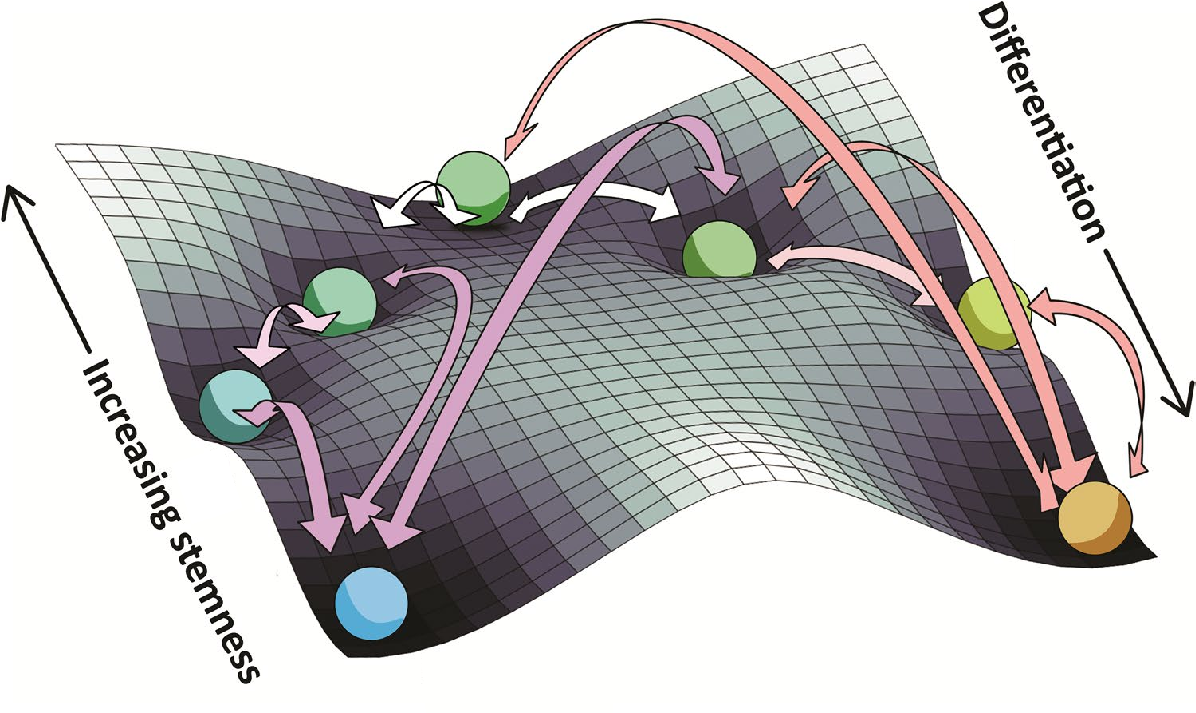
\includegraphics[width=\linewidth]{figures/WaddingtonLandscape.pdf}
            \caption{Waddington's Landscape\footnotemark[1]}
        \end{figure}
    \end{column}
    \begin{column}{0.6\textwidth}
    \begin{itemize}
        \item Cell fate determination $\equiv$ Waddington's landscape
        \item Gene regulatory networks (GRNs) regulate trajectories
        \item Master regulators - differentiation to particular state
        \item Fully differentiated - Exclusive expression (Single high)
    \end{itemize}
\end{column}
\end{columns}
\end{adjustwidth}
\footnotetext[1]{\cite{saez_dynamical_2022, furusawa_dynamical-systems_2012}. Figure by Atchuta Srinivas Duddu}
\end{frame}

\begin{frame}{Binary cell fate decision}
\begin{adjustwidth}{-5cm}{-5cm}
\begin{figure}
    \centering
    \begin{subfigure}[c]{0.3\textwidth}
        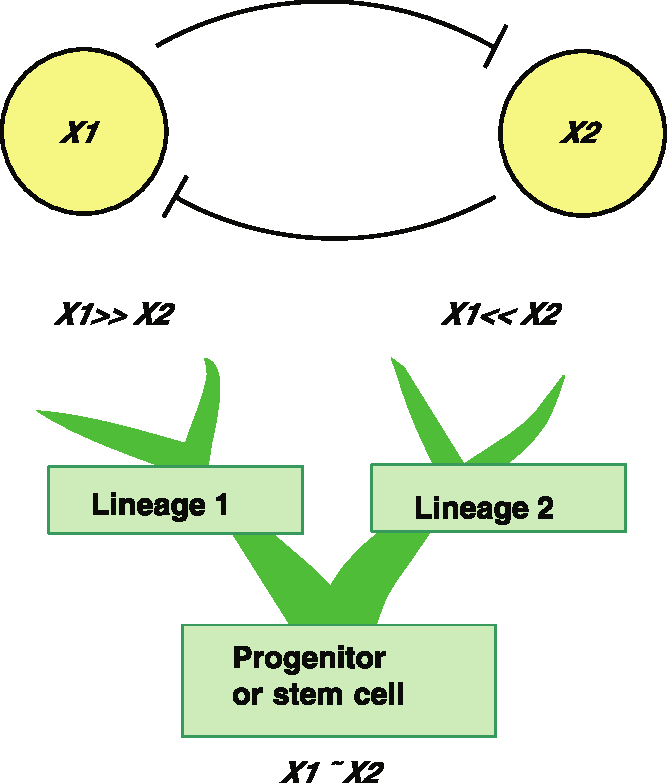
\includegraphics[width=\textwidth]{figures/ToggleSwitch.pdf}
    \end{subfigure}
    \begin{subfigure}[c]{0.7\textwidth}
        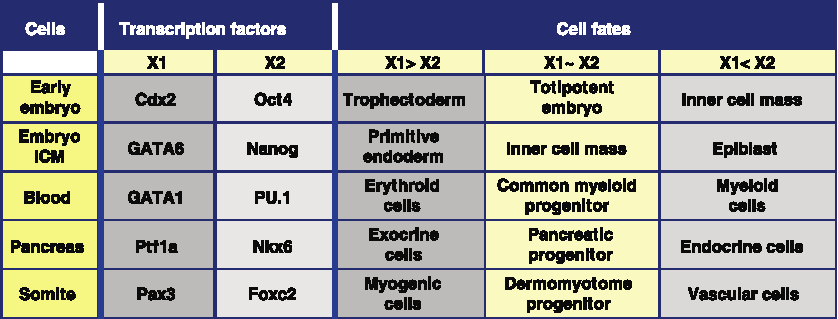
\includegraphics[width=\textwidth]{figures/ToggleSwitch_Genes.pdf}
    \end{subfigure}
    \caption{Toggle switch captures binary branching of cell fate\footnotemark[1]}
\end{figure}
\end{adjustwidth}
\footnotetext[1]{\cite{zhou_understanding_2011}}
\end{frame}

\begin{frame}{Extension to n-terminal states}
\begin{adjustwidth}{-5cm}{-5cm}
\begin{columns}
    \begin{column}{0.3\textwidth}
        \begin{figure}
        \begin{subfigure}{0.47\textwidth}
            \includesvg[width=\textwidth]{figures/Graph_T3.svg}
        \end{subfigure}
        \begin{subfigure}{0.47\textwidth}
            \includesvg[width=\textwidth]{figures/Graph_T4.svg}
        \end{subfigure}
        \begin{subfigure}{0.47\textwidth}
            \includesvg[width=\textwidth]{figures/Graph_T5.svg}
        \end{subfigure}
        \begin{subfigure}{0.47\textwidth}
            \includesvg[width=\textwidth]{figures/Graph_T6.svg}
        \end{subfigure}
        \begin{subfigure}{0.47\textwidth}
            \includesvg[width=\textwidth]{figures/Graph_T7.svg}
        \end{subfigure}
        \begin{subfigure}{0.47\textwidth}
            \includesvg[width=\textwidth]{figures/Graph_T8.svg}
        \end{subfigure}
        \caption{Toggle-n networks\footnotemark[1]}
        \end{figure}
    \end{column}
    \begin{column}{0.7\textwidth}
    \begin{figure}
        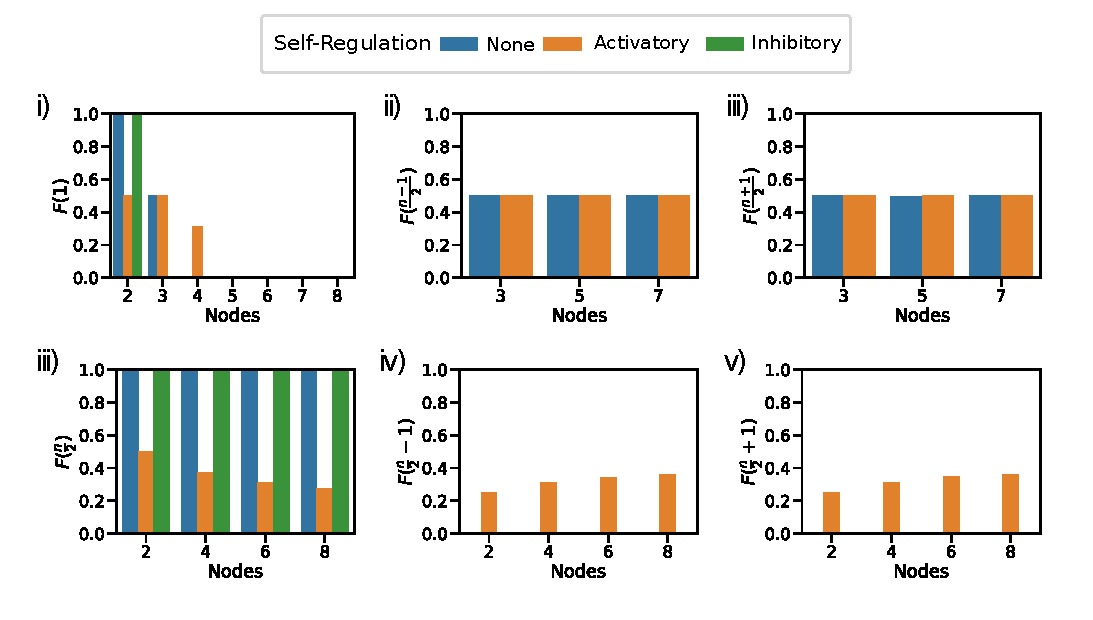
\includegraphics[width=\textwidth]{figures/Tn_General.pdf}
        \caption{Toggle-n gives n/2-high steady states\footnotemark[1]}
    \end{figure}
    \end{column}
\end{columns}
\end{adjustwidth}
\footnotetext[1]{\cite{bv_emergent_2025}}
\end{frame}

\begin{frame}[standout]
    Which networks can give rise to fully differentiated states?
    
    Single high states - only one master regulator is high
\end{frame}

\section{Methods}

\begin{frame}{Monotone Boolean Functions (MBFs)}
\begin{adjustwidth}{-5cm}{-5cm}
    \only<1>{
    \begin{figure}
        \centering
        \begin{subfigure}[c]{0.02\textwidth}
        \begin{tikzpicture}[main node/.style={circle,fill=white!20,thick,draw},scale=1.5]
                \node (1) at (0,0) {$t_1:$};
                \node (2) at (0,1) {$t_0:$};
        \end{tikzpicture}
        \end{subfigure}
        \begin{subfigure}[c]{0.25\textwidth}
            \centering
            \begin{tikzpicture}[main node/.style={circle,fill=white!20,thick,draw},scale=1.5]
                \node[main node] (1) at (0,0) {A};
                \node[main node] (2) at (1,0) {B};
                \node[main node, fill=yellow] (3) at (0,-1) {A};
                \node[main node] (4) at (1,-1) {B};
                \path[thick] (1) edge[->, color=red,shorten <= 2pt, shorten >= 2pt] (2);
                \path[thick] (3) edge[->, color=red,shorten <= 2pt, shorten >= 2pt] (4);
            \end{tikzpicture}
        \end{subfigure}
        \begin{subfigure}[c]{0.25\textwidth}
            \centering
            \begin{tikzpicture}[main node/.style={circle,fill=white!20,thick,draw},scale=1.5]
                \node[main node] (1) at (0,0) {A};
                \node[main node, fill=yellow] (2) at (1,0) {B};
                \node[main node, fill=yellow] (3) at (0,-1) {A};
                \node[main node, fill=yellow] (4) at (1,-1) {B};
                \path[thick] (1) edge[->, color=red,shorten <= 2pt, shorten >= 2pt] (2);
                \path[thick] (3) edge[->, color=red,shorten <= 2pt, shorten >= 2pt] (4);
            \end{tikzpicture}
        \end{subfigure}
        \begin{subfigure}[c]{0.25\textwidth}
            \centering
            \begin{tikzpicture}[main node/.style={circle,fill=white!20,thick,draw},scale=1.5]
                \node[main node] (1) at (0,0) {A};
                \node[main node] (2) at (1,0) {B};
                \node[main node,fill=yellow] (3) at (0,-1) {A};
                \node[main node,fill=yellow] (4) at (1,-1) {B};
                \path[thick] (1) edge[->, color=red,shorten <= 2pt, shorten >= 2pt] (2);
                \path[thick] (3) edge[->, color=red,shorten <= 2pt, shorten >= 2pt] (4);
            \end{tikzpicture}
        \end{subfigure}
        \begin{subfigure}[c]{0.2\textwidth}
            \centering
            \begin{tikzpicture}[main node/.style={circle,fill=white!20,thick,draw},scale=1.5]
                \node[main node] (1) at (0,0) {A};
                \node[main node,fill=yellow] (2) at (1,0) {B};
                \node[main node,fill=yellow] (3) at (0,-1) {A};
                \node[main node] (4) at (1,-1) {B};
                \path[thick] (1) edge[->, color=red,shorten <= 2pt, shorten >= 2pt] (2);
                \path[thick] (3) edge[->, color=red,shorten <= 2pt, shorten >= 2pt] (4);
                \draw[red, ultra thick] (-0.3,0.3) -- (1.3,-1.3);
                \draw[red, ultra thick] (-0.3,-1.3) -- (1.3,0.3);
            \end{tikzpicture}
        \end{subfigure}
        \pause[1]\caption{Schematic of increasing MBF(1) for activatory input}
    \end{figure}}
    \only<2>{
    \begin{figure}
        \centering
        \begin{subfigure}[c]{0.02\textwidth}
        \begin{tikzpicture}[main node/.style={circle,fill=white!20,thick,draw},scale=1.5]
                \node (1) at (0,0) {$t_1:$};
                \node (2) at (0,1) {$t_0:$};
        \end{tikzpicture}
        \end{subfigure}
        \begin{subfigure}[c]{0.25\textwidth}
            \centering
            \begin{tikzpicture}[main node/.style={circle,fill=white!20,thick,draw},scale=1.5]
                \node[main node] (1) at (0,0) {A};
                \node[main node] (2) at (1,0) {B};
                \node[main node, fill=yellow] (3) at (0,-1) {A};
                \node[main node] (4) at (1,-1) {B};
                \path[thick] (1) edge[-|, color=blue,shorten <= 2pt, shorten >= 2pt] (2);
                \path[thick] (3) edge[-|, color=blue,shorten <= 2pt, shorten >= 2pt] (4);
            \end{tikzpicture}
        \end{subfigure}
        \begin{subfigure}[c]{0.25\textwidth}
            \centering
            \begin{tikzpicture}[main node/.style={circle,fill=white!20,thick,draw},scale=1.5]
                \node[main node] (1) at (0,0) {A};
                \node[main node, fill=yellow] (2) at (1,0) {B};
                \node[main node, fill=yellow] (3) at (0,-1) {A};
                \node[main node, fill=yellow] (4) at (1,-1) {B};
                \path[thick] (1) edge[-|, color=blue,shorten <= 2pt, shorten >= 2pt] (2);
                \path[thick] (3) edge[-|, color=blue,shorten <= 2pt, shorten >= 2pt] (4);
            \end{tikzpicture}
        \end{subfigure}
        \begin{subfigure}[c]{0.25\textwidth}
            \centering
            \begin{tikzpicture}[main node/.style={circle,fill=white!20,thick,draw},scale=1.5]
                \node[main node] (1) at (0,0) {A};
                \node[main node, fill=yellow] (2) at (1,0) {B};
                \node[main node, fill=yellow] (3) at (0,-1) {A};
                \node[main node] (4) at (1,-1) {B};
                \path[thick] (1) edge[-|, color=blue,shorten <= 2pt, shorten >= 2pt] (2);
                \path[thick] (3) edge[-|, color=blue,shorten <= 2pt, shorten >= 2pt] (4);
            \end{tikzpicture}
        \end{subfigure}
        \begin{subfigure}[c]{0.25\textwidth}
            \centering
            \begin{tikzpicture}[main node/.style={circle,fill=white!20,thick,draw},scale=1.5]
                \node[main node] (1) at (0,0) {A};
                \node[main node] (2) at (1,0) {B};
                \node[main node,fill=yellow] (3) at (0,-1) {A};
                \node[main node,fill=yellow] (4) at (1,-1) {B};
                \path[thick] (1) edge[-|, color=blue,shorten <= 2pt, shorten >= 2pt] (2);
                \path[thick] (3) edge[-|, color=blue,shorten <= 2pt, shorten >= 2pt] (4);
                \draw[red, ultra thick] (-0.3,0.3) -- (1.3,-1.3);
                \draw[red, ultra thick] (-0.3,-1.3) -- (1.3,0.3);
            \end{tikzpicture}
        \end{subfigure}
        \caption{Schematic of decreasing MBF(1) for inhibitory input}
    \end{figure}}
    \only<3>{
    \begin{figure}
        \centering
        \begin{subfigure}[c]{0.2\textwidth}
            \centering
            \begin{tikzpicture}[main node/.style={circle,fill=white!20,thick,draw},scale=1.5]
                \node[main node] (1) at (0,1) {X};
                \node[main node] (2) at (0,0) {Y};
                \node[main node] (3) at (1,0.5) {Z};
                \path[thick] (1) edge[->, color=red,shorten <= 2pt, shorten >= 2pt] (3);
                \path[thick] (2) edge[->, color=red,shorten <= 2pt, shorten >= 2pt] (3);
            \end{tikzpicture}
        \end{subfigure}
        \begin{subfigure}[c]{0.4\textwidth}
            \centering
            \begin{tabular}{|c|c|c|c|c|c|c|c|}
            \hline
            \multicolumn{2}{|c|}{\textbf{Inputs}} & \multicolumn{6}{|c|}{\textbf{MBFs}} \\ \hline
            $X$ & $Y$ & $\bzero$ & $\wedge$ & ${\bf X}$ & ${\bf Y}$ & $\vee$ & $\bone$ \\ \hline
            0 & 0 & 0 & 0 & 0 & 0 & 0 & 1 \\
            0 & 1 & 0 & 0 & 0 & 1 & 1 & 1 \\
            1 & 0 & 0 & 0 & 1 & 0 & 1 & 1 \\
            1 & 1 & 0 & 1 & 1 & 1 & 1 & 1 \\ \hline
            \end{tabular}
        \end{subfigure}
        \caption{Table of MBF(2) for a node with two activatory inputs $X$ and $Y$.}
    \end{figure}
    }
\end{adjustwidth}
\footnotetext[1]{\cite{korshunov_monotone_2003}}
\end{frame}

% \begin{frame}[noframenumbering]{MBF(2)}
% \only<1-2>{
% \begin{table}[h!]
% \centering
% \only<1>{
% \begin{tabular}{|c|c|c|c|c|c|c|c|c|c|c|c|c|c|c|c|c|c|}
% \hline
% \multicolumn{2}{|c|}{\textbf{Inputs}} & \multicolumn{16}{|c|}{\textbf{BFs}}\\ \hline
% $X$ & $Y$ & \multicolumn{16}{|c|}{}\\ \hline
% 0 & 0 & 0 & 0 & 0 & 0 & 0 & 0 & 0 & 0 & 1 & 1 & 1 & 1 & 1 & 1 & 1 & 1 \\
% 0 & 1 & 0 & 0 & 0 & 0 & 1 & 1 & 1 & 1 & 0 & 0 & 0 & 0 & 1 & 1 & 1 & 1 \\
% 1 & 0 & 0 & 0 & 1 & 1 & 0 & 0 & 1 & 1 & 0 & 0 & 1 & 1 & 0 & 0 & 1 & 1 \\
% 1 & 1 & 0 & 1 & 0 & 1 & 0 & 1 & 0 & 1 & 0 & 1 & 0 & 1 & 0 & 1 & 0 & 1 \\ \hline
% \end{tabular}}
% \only<2>{
% \begin{tabular}{|c|c|c|c|c|c|c|c|c|c|c|c|c|c|c|c|c|c|}
% \hline
% \multicolumn{2}{|c|}{\textbf{Inputs}} & \multicolumn{16}{|c|}{\textbf{BFs}}\\ \hline
% $X$ & $Y$ & \multicolumn{16}{|c|}{}\\ \hline
% 0 & 0 & 0 & 0 & \red{0} & 0 & \red{0} & 0 & \red{0} & 0 & \red{1} & \red{1} & \red{1} & \red{1} & \red{1} & \red{1} & \red{1} & 1 \\
% 0 & 1 & 0 & 0 & \red{0} & 0 & \red{1} & 1 & \red{1} & 1 & \red{0} & \red{0} & \red{0} & \red{0} & \red{1} & \red{1} & \red{1} & 1 \\
% \textbf{1} & \textbf{0} & 0 & 0 & \textbf{\red{1}} & 1 & \red{0} & 0 & \red{1} & 1 & \red{0} & \red{0} & \red{1} & \red{1} & \red{0} & \red{0} & \red{1} & 1 \\
% \textbf{1} & \textbf{1} & 0 & 1 & \textbf{\red{0}} & 1 & \red{0} & 1 & \red{0} & 1 & \red{0} & \red{1} & \red{0} & \red{1} & \red{0} & \red{1} & \red{0} & 1 \\ \hline
% \end{tabular}}
% \caption{Table of BFs for a node with two inputs $X$ and $Y$.}
% \end{table}}
% \only<2>{\footnotetext[1]{Red indicates non-increasing functions (non-monotonous)}}
% \only<3>{

% \begin{frame}{MBF(2)}
% \begin{figure}[t]
%     \centering
%     \begin{subfigure}[c]{0.5\textwidth}
%         \centering
%         \begin{tabular}{|c|c|c|c|c|c|c|c|}
%         \hline
%         \multicolumn{2}{|c|}{\textbf{Inputs}} & \multicolumn{6}{|c|}{\textbf{MBFs}} \\ \hline
%         $X$ & $Y$ & $\bzero$ & $\wedge$ & ${\bf X}$ & ${\bf Y}$ & $\vee$ & $\bone$ \\ \hline
%         0 & 0 & 0 & 0 & 0 & 0 & 0 & 1 \\
%         0 & 1 & 0 & 0 & 0 & 1 & 1 & 1 \\
%         1 & 0 & 0 & 0 & 1 & 0 & 1 & 1 \\
%         1 & 1 & 0 & 1 & 1 & 1 & 1 & 1 \\ \hline
%         \end{tabular}
%     \end{subfigure}
%     \begin{subfigure}{0.3\textwidth}
%         \begin{tikzpicture}[node distance = .5cm,baseline=(current bounding box.center)]
%             \tikzset{my node/.style = {circle, draw, thick, inner sep=4pt, minimum size=0pt}}
%             \tikzset{my edge/.style = {-, very thick}}
%             \node[my node] (1) { $\bone$ };
%             \node[my node] (2) [below=of 1] {$\vee$};
%             \node[my node] (3) [below left=0.4 and 0.2 of 2] {$X$};
%             \node[my node] (4) [below right=0.4 and 0.2 of 2] {$Y$};
%             \node[my node] (5) [below left=0.4 and 0.2 of 4] {$\wedge$};
%             \node[my node] (6) [below=of 5] {$\bzero$};
%             \draw[my edge] (1) -- (2);
%             \draw[my edge] (2) -- (3);
%             \draw[my edge] (2) -- (4);
%             \draw[my edge] (3) -- (5);
%             \draw[my edge] (4) -- (5);
%             \draw[my edge] (5) -- (6);
%         \end{tikzpicture}
%     \end{subfigure}
% \caption{Table (left) and Lattice (right) of MBF(2) for a node with two activatory inputs $X$ and $Y$.}
% \end{figure}
% \end{frame}

% \begin{frame}{Lattice}
    
% \end{frame}

\begin{frame}{Up-sets and Down-sets}
\begin{adjustwidth}{-5cm}{-5cm}
\begin{columns}
    \begin{column}{0.4\textwidth}
        \begin{align*}
            U(b) &:=\{ f\in MBF(s) \;|\; f(b) = 1\} \\
            L(b) &:=\{ f\in MBF(s) \;|\; f(b) = 0\}.
        \end{align*}
        \vspace{0.5cm}
        
        \pause[3]Lattice theory:
        \begin{itemize}
            \item $U$s = prime ideals
            \item $L$s = prime filters
        \end{itemize}
    \end{column}
    \pause[2]
    \begin{column}{0.6\textwidth}
        \begin{figure}
        \begin{subfigure}[c]{0.59\textwidth}
        \begin{tabular}{|c|c|c|}
         \hline 
         L(11)  & $\{\bzero\}$                    &1 \\
         L(10)  & $\{\bzero, \wedge, Y\}$         &3 \\
         L(01)  & $\{\bzero, \wedge, X\}$         &3 \\
         L(00)  & $\{\bzero, \wedge, X, Y,\vee\}$ &5 \\
         \hline
         \hline
         U(11) &  $\{\bone, \vee, X, Y, \wedge\}$ &5 \\
         U(10) &  $\{\bone, \vee, X \}$           &3 \\
         U(01) &  $\{\bone, \vee, Y\}$            &3 \\
         U(00) &  $\{\bone\}$                     &1 \\
         \hline
        \end{tabular}
        \end{subfigure}
        \pause[3]
        \begin{subfigure}[c]{0.39\textwidth}
            \begin{tikzpicture}[node distance = .3cm,baseline=(current bounding box.center)]
                \tikzset{my node/.style = {circle, draw, fill=none, very thick, inner sep=4pt, minimum size=0pt}}
                \tikzset{my edge/.style = {-, very thick}}
                \node[my node, dashed] (1) { $\bone$ };
                \node[my node, red] (2) [below=of 1] {$\vee$};
                \node[my node, red, dashed] (3) [below left=0.4 and 0.2 of 2] {$X$};
                \node[my node, red, dashed] (4) [below right=0.4 and 0.2 of 2] {$Y$};
                \node[my node, dashed] (5) [below left=0.4 and 0.2 of 4] {$\wedge$};
                \node[my node, red] (6) [below=of 5] {$\bzero$};
                \draw[my edge] (1) -- (2);
                \draw[my edge] (2) -- (3);
                \draw[my edge] (2) -- (4);
                \draw[my edge] (3) -- (5);
                \draw[my edge] (4) -- (5);
                \draw[my edge] (5) -- (6);
            \end{tikzpicture}
        \end{subfigure}
        \pause[2]\caption{$U$ and $L$ for $MBF(2)$}
        \end{figure}
    \end{column}
\end{columns}
\end{adjustwidth}
\footnotetext[1]{$b\in \bbB^s$; $s=$ No. of inputs; Dashed lines indicate prime ideals, Red lines indicate prime filters}
\footnotetext[2]{\cite{adigwe_characterization_2026}}
\end{frame}

\begin{frame}{Steady states}
\begin{columns}
    \begin{column}{0.5\textwidth}
        Network $N=(V,E,\delta)$

        Boolean models $f=(f_1,f_2, \ldots, f_n)$
    \end{column}
    \begin{column}{0.5\textwidth}
        Boolean state $b=(b_1, \ldots, b_n)\in \bbB^n$

        Steady state $\implies f(b) = b$
    \end{column}
\end{columns}
    \[ f_i \in I_i(\beta_i(b))\]
    where,
    \[ I_i(b)= \left\{ \begin{array}{cc}
    U(\beta_i(b_{\Sources(i)})) & \mbox{ if } \quad b_i=1\\
    L(\beta_i(b_{\Sources(i)})) &\mbox{ if } \quad b_i=0
    \end{array}
    \right .
    \]

    \[ \beta^j_i = \left \{
    \begin{array}{cc}
    Id & \mbox{ if } \delta(j,i)=1\\
    \neg Id &  \mbox{ if } \delta(j,i)=-1
    \end{array}
    \right.
    .\]
\footnotetext[1]{ $b_{\Sources(i)}=$  values of the inputs of node $i$ evaluated at the state $b$}
\footnotetext[2]{\cite{adigwe_characterization_2026}}
\end{frame}

\begin{frame}{Multistability}

    Steady states:  $b^1,\ldots, b^q \in \bbB^n$
    \[ f_i \in \bigcap_{j=1}^q I_i(b^j)\]
    where,
    \[ I_i(b^k)= \left\{ \begin{array}{cc}
    U(\beta_i(b^k_{\Sources(i)})) & \mbox{ if } \quad  b^k_i=1\\
    L(\beta_i(b^k_{\Sources(i)})) &\mbox{ if } \quad  b^k_i=0
    \end{array}
    \right . 
    \]

    \[ \beta^j_i = \left \{
    \begin{array}{cc}
    Id & \mbox{ if } \delta(j,i)=1\\
    \neg Id &  \mbox{ if } \delta(j,i)=-1
    \end{array}
    \right.
    .\]
    
\footnotetext[1]{$b^k_{\Sources(i)}=$ values of the inputs of node $i$ evaluated at the state $b^k$}
\footnotetext[2]{\cite{adigwe_characterization_2026}}
\end{frame}

\section{Results}

\begin{frame}[standout]
    Which network(s) have the maximum prevalence of single high states?
\end{frame}

\begin{frame}{Team networks maximize prevalance of one single high state}
\begin{adjustwidth}{-5cm}{-5cm}
\begin{columns}
    \begin{column}{0.3\textwidth}
        Most MBMs for $e \in \bbB^n$ 
        \[ H = \prod_{i=1}^n (|MBF(s_i)|-1). \]
        \[|L(\bzero^s)| = |U(\bone^s)| = |MBF(s)| -1\]
        
        \pause \[e^1 = (10\ldots0) \text{ with } H \text{ MBMs }\]
        \pause \[U(\beta_1(10\ldots0)) \rightarrow U(11\ldots1)\]     
        \pause \[L(\beta_j(10\ldots0)) \rightarrow L(00\ldots0)\]
    \end{column}
    \pause[1]
    \begin{column}{0.7\textwidth}
    \only<2>{\begin{figure}[h!]
    \centering
    \begin{subfigure}{0.25\textwidth}
        \centering
        \begin{tikzpicture}[scale=2]
            \node[main node] (A) at (0,0) {A};
            \node[main node] (B) at (0,-1) {B};
            \path[blankedge]
                (A) edge[bend left] (B)
                (B) edge[bend left] (A)
                (A) edge[loop above] (A)
                (B) edge[loop below] (B)
                ;
        \end{tikzpicture}
        \caption{(10) (01)}
        \label{fig:TS}
    \end{subfigure}
    \begin{subfigure}{0.33\textwidth}
        \centering
        \begin{tikzpicture}[scale=2]
            \node[main node] (A) at (0.5,0.86) {A};
            \node[main node] (B) at (0,0) {B};
            \node[main node] (C) at (1,0) {C};
            \path[blankedge]
                (A) edge (B)
                (A) edge[bend left] (C)
                (B) edge[bend left] (A)
                (C) edge (A)
                (B) edge (C)
                (C) edge[bend left] (B)
                (A) edge[loop above] (A)
                (B) edge[in=240, out=270,looseness=3,min distance=3mm] (B)
                (C) edge[in=270, out=300,looseness=3,min distance=3mm] (C)
                ;
        \end{tikzpicture}
        \caption{(100)}
        \label{fig:3TeamA}
    \end{subfigure}
    \begin{subfigure}{0.33\textwidth}
        \centering
        \begin{tikzpicture}[scale=2]
            \node[main node] (A) at (0,0.85) {A};
            \node[main node] (B) at (0,0) {B};
            \node[main node] (C) at (0.85,0) {C};
            \node[main node] (D) at (0.85,0.85) {D};
            \path[blankedge]
                (A) edge (B)
                (A) edge[bend left=15, shorten <=6pt] (C)
                (A) edge[bend left] (D)
                (B) edge[bend left] (A)
                (C) edge[bend left=15, shorten <=6pt] (A)
                (D) edge (A)
                (B) edge (C)
                (B) edge[bend left=15, shorten <=6pt] (D)
                (C) edge[bend left] (B)
                (C) edge (D)
                (D) edge[bend left=15, shorten <=6pt] (B)
                (D) edge[bend left] (C)
                (A) edge[in=120, out=150,looseness=3,min distance=3mm] (A)
                (B) edge[in=210, out=240,looseness=3,min distance=3mm] (B)
                (C) edge[in=300, out=330,looseness=3,min distance=3mm] (C)
                (D) edge[in=30, out=60,looseness=3,min distance=3mm] (D)
                ;
        \end{tikzpicture}
        \caption{(1000)}
        \label{fig:4TeamA}
    \end{subfigure}
    \caption{Network structures with $H$ MBMs supporting $e^1$}
    \end{figure}
    }\only<3>{
    \begin{figure}[h!]
    \centering
    \begin{subfigure}{0.25\textwidth}
        \centering
        \begin{tikzpicture}[scale=2]
            \node[main node] (A) at (0,0) {A};
            \node[main node] (B) at (0,-1) {B};
            \path[blueedge]
                (B) edge[bend left] (A);
            \path[rededge]
                (A) edge[loop above] (A);
            \path[blankedge]
                (A) edge[bend left] (B)
                (B) edge[loop below] (B)
                ;
        \end{tikzpicture}
        \caption{(10)}
        \label{fig:TS}
    \end{subfigure}
    \begin{subfigure}{0.33\textwidth}
        \centering
        \begin{tikzpicture}[scale=2]
            \node[main node] (A) at (0.5,0.86) {A};
            \node[main node] (B) at (0,0) {B};
            \node[main node] (C) at (1,0) {C};
            \path[blankedge]
                (A) edge (B)
                (A) edge[bend left] (C)
                (B) edge (C)
                (C) edge[bend left] (B)
                (B) edge[in=240, out=270,looseness=3,min distance=3mm] (B)
                (C) edge[in=270, out=300,looseness=3,min distance=3mm] (C)
                ;
            \path[blueedge]
                (B) edge[bend left] (A)
                (C) edge (A)
                ;
            \path[rededge]
                (A) edge[loop above] (A);
        \end{tikzpicture}
        \caption{(100)}
        \label{fig:3TeamA}
    \end{subfigure}
    \begin{subfigure}{0.33\textwidth}
        \centering
        \begin{tikzpicture}[scale=2]
            \node[main node] (A) at (0,0.85) {A};
            \node[main node] (B) at (0,0) {B};
            \node[main node] (C) at (0.85,0) {C};
            \node[main node] (D) at (0.85,0.85) {D};
            \path[blankedge]
                (A) edge (B)
                (A) edge[bend left=15, shorten <=6pt] (C)
                (A) edge[bend left] (D)
                (B) edge (C)
                (B) edge[bend left=15, shorten <=6pt] (D)
                (C) edge[bend left] (B)
                (C) edge (D)
                (D) edge[bend left=15, shorten <=6pt] (B)
                (D) edge[bend left] (C)
                (B) edge[in=210, out=240,looseness=3,min distance=3mm] (B)
                (C) edge[in=300, out=330,looseness=3,min distance=3mm] (C)
                (D) edge[in=30, out=60,looseness=3,min distance=3mm] (D)
                ;
            \path[blueedge]
                (B) edge[bend left] (A)
                (C) edge[bend left=15, shorten <=6pt] (A)
                (D) edge (A)
                ;
            \path[rededge]
                (A) edge[in=120, out=150,looseness=3,min distance=3mm] (A);
        \end{tikzpicture}
        \caption{(1000)}
        \label{fig:4TeamA}
    \end{subfigure}
    \caption{Network structures with $H$ MBMs supporting $e^1$}
    \end{figure}
    }\only<4->{
    \begin{figure}[h!]
    \centering
    \begin{subfigure}{0.25\textwidth}
        \centering
        \begin{tikzpicture}[scale=2]
            \node[main node] (A) at (0,0) {A};
            \node[main node] (B) at (0,-1) {B};
            \path[blueedge]
                (A) edge[bend left] (B)
                (B) edge[bend left] (A)
                ;
            \path[rededge]
                (A) edge[loop above] (A)
                (B) edge[loop below] (B)
                ;
        \end{tikzpicture}
        \caption{(10)}
        \label{fig:TS}
    \end{subfigure}
    \begin{subfigure}{0.33\textwidth}
        \centering
        \begin{tikzpicture}[scale=2]
            \node[main node] (A) at (0.5,0.86) {A};
            \node[main node] (B) at (0,0) {B};
            \node[main node] (C) at (1,0) {C};
            \path[blueedge]
                (A) edge (B)
                (A) edge[bend left] (C)
                (B) edge[bend left] (A)
                (C) edge (A)
                ;
            \path[rededge]
                (B) edge (C)
                (C) edge[bend left] (B)
                (A) edge[loop above] (A)
                (B) edge[in=240, out=270,looseness=3,min distance=3mm] (B)
                (C) edge[in=270, out=300,looseness=3,min distance=3mm] (C)
                ;
        \end{tikzpicture}
        \caption{(100)}
        \label{fig:3TeamA}
    \end{subfigure}
    \begin{subfigure}{0.33\textwidth}
        \centering
        \begin{tikzpicture}[scale=2]
            \node[main node] (A) at (0,0.85) {A};
            \node[main node] (B) at (0,0) {B};
            \node[main node] (C) at (0.85,0) {C};
            \node[main node] (D) at (0.85,0.85) {D};
            \path[blueedge]
                (A) edge (B)
                (A) edge[bend left=15, shorten <=6pt] (C)
                (A) edge[bend left] (D)
                (B) edge[bend left] (A)
                (C) edge[bend left=15, shorten <=6pt] (A)
                (D) edge (A)
                ;
            \path[rededge]
                (B) edge (C)
                (B) edge[bend left=15, shorten <=6pt] (D)
                (C) edge[bend left] (B)
                (C) edge (D)
                (D) edge[bend left=15, shorten <=6pt] (B)
                (D) edge[bend left] (C)
                (A) edge[in=120, out=150,looseness=3,min distance=3mm] (A)
                (B) edge[in=210, out=240,looseness=3,min distance=3mm] (B)
                (C) edge[in=300, out=330,looseness=3,min distance=3mm] (C)
                (D) edge[in=30, out=60,looseness=3,min distance=3mm] (D)
                ;
        \end{tikzpicture}
        \caption{(1000)}
        \label{fig:4TeamA}
    \end{subfigure}
    \caption{Network structures with $H$ MBMs supporting $e^1$}
    \end{figure}}
    \end{column}
\end{columns}
\end{adjustwidth}
\footnotetext[1]{$s_i = $ No. of inputs to node $i$; $\bzero^s(\bone^s)= $ vectors of zeros(ones) $\in \bbB^s$; $e^k = k$-th unit vector $\in \bbB^n$}
\footnotetext[2]{\cite{adigwe_characterization_2026}}
\footnotetext[3]{\cite{bv_gene_2026}}
\end{frame}

\begin{frame}{Disconnected networks maximize all single high states}
\begin{adjustwidth}{-5cm}{-5cm}
\begin{columns}
    \begin{column}{0.25\textwidth}
        \[e^i \text{ with } H \text{ MBMs }\]
        \pause
        \[e^j \text{ with } H \text{ MBMs }\]
        
        \pause 
        \[\text{Disconnected networks}\]
        \[\text{Domain of attraction}(e^i) = \{e^i\}\]
    \end{column}
    \pause[1]
    \begin{column}{0.7\textwidth}
    \only<1>{
    \begin{figure}[h!]
    \centering
    \begin{subfigure}{0.49\textwidth}
        \centering
        \begin{tikzpicture}[scale=2]
            \node[main node] (A) at (0.4,0.67) {A};
            \node[main node] (B) at (0,0) {B};
            \node[main node] (C) at (0.8,0) {C};
            \path[rededge]
                (A) edge[loop above] (A)
                (B) edge[in=195, out=225,loop] (B)
                (C) edge[in=315, out=345,loop] (C)
                ;
            \path[blueedge]
                (A) edge (B)
                (A) edge[bend left] (C)
                (B) edge[bend left] (A)
                (C) edge (A)
                ;
            \path[rededge]
                (B) edge (C)
                (C) edge[bend left] (B)
                ;
        \end{tikzpicture}
        \caption{(100)\textcolor{gray}{(010)(001)}}
        \label{fig:3Disc}
    \end{subfigure}
    \begin{subfigure}{0.49\textwidth}
        \centering
        \begin{tikzpicture}[scale=2]
            \node[main node] (A) at (0,0.75) {A};
            \node[main node] (B) at (0,0) {B};
            \node[main node] (C) at (0.75,0) {C};
            \node[main node] (D) at (0.75,0.75) {D};
            \path[rededge]
                (A) edge[in=120, out=150,loop] (A)
                (B) edge[in=210, out=240,loop] (B)
                (C) edge[in=300, out=330,loop] (C)
                (D) edge[in=30, out=60,loop] (D)
                ;
            \path[blueedge]
                (A) edge (B)
                (A) edge[bend left=15, shorten <=6pt] (C)
                (A) edge[bend left] (D)
                (B) edge[bend left] (A)
                (C) edge[bend left=15, shorten <=6pt] (A)
                (D) edge (A)
                ;
            \path[rededge]
                (B) edge (C)
                (B) edge[bend left=15, shorten <=6pt] (D)
                (C) edge[bend left] (B)
                (C) edge (D)
                (D) edge[bend left=15, shorten <=6pt] (B)
                (D) edge[bend left] (C)
                ;
        \end{tikzpicture}
        \caption{(1000)\textcolor{gray}{(0100)(0010)(0001)}}
        \label{fig:4Disc}
    \end{subfigure}
    \caption{Network structures with $H$ MBMs supporting $e^1,\ldots,e^n$}
    \end{figure}
    }\only<2>{
    \begin{figure}[h!]
    \centering
    \begin{subfigure}{0.49\textwidth}
        \centering
        \begin{tikzpicture}[scale=2]
            \node[main node] (A) at (0.4,0.67) {A};
            \node[main node] (B) at (0,0) {B};
            \node[main node] (C) at (0.8,0) {C};
            \path[rededge]
                (A) edge[loop above] (A)
                (B) edge[in=195, out=225,loop] (B)
                (C) edge[in=315, out=345,loop] (C)
                ;
            \path[blueedge, opacity=0.2]
                (A) edge (B)
                (A) edge[bend left] (C)
                (B) edge[bend left] (A)
                (C) edge (A)
                ;
            \path[rededge, opacity=0.2]
                (B) edge (C)
                (C) edge[bend left] (B)
                ;
            \path[rededge]
                (A) edge[bend left=50] (C)
                (C) edge[bend right=10] (A)
                ;
            \path[blueedge]
                (A) edge[bend right=10] (B)
                (B) edge[bend left=50] (A)
                (B) edge[bend right=10] (C)
                (C) edge[bend left=50] (B)
                ;
        \end{tikzpicture}
        \caption{\textcolor{gray}{(100)}(010)\textcolor{gray}{(001)}}
        \label{fig:3Disc}
    \end{subfigure}
    \begin{subfigure}{0.49\textwidth}
        \centering
        \begin{tikzpicture}[scale=2]
            \node[main node] (A) at (0,0.75) {A};
            \node[main node] (B) at (0,0) {B};
            \node[main node] (C) at (0.75,0) {C};
            \node[main node] (D) at (0.75,0.7) {D};
            \path[rededge]
                (A) edge[in=120, out=150,loop] (A)
                (B) edge[in=210, out=240,loop] (B)
                (C) edge[in=300, out=330,loop] (C)
                (D) edge[in=30, out=60,loop] (D)
                ;
            \path[blueedge,opacity=0.2]
                (A) edge (B)
                (A) edge[bend left=15, shorten <=6pt] (C)
                (A) edge[bend left] (D)
                (B) edge[bend left] (A)
                (C) edge[bend left=15, shorten <=6pt] (A)
                (D) edge (A)
                ;
            \path[rededge,opacity=0.2]
                (B) edge (C)
                (B) edge[bend left=15, shorten <=6pt] (D)
                (C) edge[bend left] (B)
                (C) edge (D)
                (D) edge[bend left=15, shorten <=6pt] (B)
                (D) edge[bend left] (C)
                ;
            \path[blueedge]
                (A) edge[bend right=10] (B)
                (B) edge[bend left=45] (A)
                (B) edge[bend right=10] (C)
                (C) edge[bend left=45] (B)
                (B) edge[bend left=10, shorten <=6pt] (D)
                (D) edge[bend left=10, shorten <=6pt] (B)
                ;
            \path[rededge]
                (A) edge[bend left=20, shorten <=6pt] (C)
                (A) edge[bend left=45] (D)
                (C) edge[bend left=20, shorten <=6pt] (A)
                (D) edge[bend right=10] (A)
                (C) edge[bend right=10] (D)
                (D) edge[bend left=45] (C)
                ;
        \end{tikzpicture}
        \caption{\textcolor{gray}{(1000)}(0100)\textcolor{gray}{(0010)(0001)}}
        \label{fig:4Disc}
    \end{subfigure}
    \caption{Network structures with $H$ MBMs supporting $e^1,\ldots,e^n$}
    \end{figure}
    }\only<3->{
    \begin{figure}[h!]
    \centering
    \begin{subfigure}{0.49\textwidth}
        \centering
        \begin{tikzpicture}[scale=2]
            \node[main node] (A) at (0.4,0.67) {A};
            \node[main node] (B) at (0,0) {B};
            \node[main node] (C) at (0.8,0) {C};
            \path[rededge]
                (A) edge[loop above] (A)
                (B) edge[in=195, out=225,loop] (B)
                (C) edge[in=315, out=345,loop] (C)
                ;
        \end{tikzpicture}
        \caption{(100)(010)(001)}
        \label{fig:3Disc}
    \end{subfigure}
    \begin{subfigure}{0.49\textwidth}
        \centering
        \begin{tikzpicture}[scale=2]
            \node[main node] (A) at (0,0.75) {A};
            \node[main node] (B) at (0,0) {B};
            \node[main node] (C) at (0.75,0) {C};
            \node[main node] (D) at (0.75,0.75) {D};
            \path[rededge]
                (A) edge[in=120, out=150,loop] (A)
                (B) edge[in=210, out=240,loop] (B)
                (C) edge[in=300, out=330,loop] (C)
                (D) edge[in=30, out=60,loop] (D)
                ;
        \end{tikzpicture}
        \caption{(1000)(0100)(0010)(0001)}
        \label{fig:4Disc}
    \end{subfigure}
    \caption{Network structures with $H$ MBMs supporting $e^1,\ldots,e^n$}
    \end{figure}
    }
\end{column}
\end{columns}
\pause[4]
\begin{center}
    Network without mutual communication cannot serve as decision network
\end{center}
\end{adjustwidth}
\footnotetext[1]{$e^k = k$-th unit vector $\in \bbB^n$}
\footnotetext[2]{\cite{bv_gene_2026}}
\end{frame}

\begin{frame}[standout]
    Which network(s) have equal prevalance of single high states? \\ (Equipotent networks)

    Which among them have the most number of models?
\end{frame}

\begin{frame}{Equipotent networks}
    \pause[3]Consider networks with all-to-all coupling without self-edges 
    \pause[1]
    \only<1-2>{
    \[
    \begin{array}{c|ccccc}
     & f_1 & f_2 & \cdots & f_n \\
    \hline
    e^1 &
    |U(\beta_1(e^1_{\Sources(1)}))| &
    |L(\beta_2(e^1_{\Sources(2)}))| &
    \cdots &
     % |L(\beta_{n-1}(e^1_{\Sources(n-1)}))| &
     |L(\beta_n(e^1_{\Sources(n)}))|
    \\
    e^2 &
    |L(\beta_1(e^2_{\Sources(1)}))|&
    |U(\beta_2(e^2_{\Sources(2)}))| &
    \cdots &
    % |L(\beta_{n-1}(e^2_{\Sources(n-1)}))| &
    |L(\beta_n(e^2_{\Sources(n)}))|
    \\
    \vdots & \vdots & \vdots & \ddots & \vdots & \vdots
    \\
    e^n &
    |L(\beta_1(e^n_{\Sources(1)}))| &
    |L(\beta_2(e^n_{\Sources(2)}))|&
    \cdots &
    % |L(\beta_{n-1}(e^n_{\Sources(n-1)}))|&
    |U(\beta_n(e^n_{\Sources(n)}))|
    \end{array}.
    \]
    }\only<3->{
        \[
    \begin{array}{c|ccccc}
     & f_1 & f_2 & \cdots  & f_n \\
    \hline
    e^1 &
    |U(\beta_1(\bzero^{n-1}))| &
    |L(\beta_2(e^{1,n-1}))| &
    \cdots &
     % |L(\beta_{n-1}(e^{1,n-1)}))| &
     |L(\beta_n(e^{1,n-1)}))|
    \\
    e^2 &
    |L(\beta_1(e^{1,n-1)}))|&
    |U(\beta_2(\bzero^{n-1}))| &
    \cdots &
    % |L(\beta_{n-1}(e^{2,n-1)}))| &
    |L(\beta_n(e^{2,n-1)}))|
    \\
    \vdots & \vdots & \vdots & \ddots & \vdots & \vdots
    \\
    e^n &
    |L(\beta_1(e^{n-1,n-1)}))| &
    |L(\beta_2(e^{n-1,n-1)}))|&
    \cdots &
    % |L(\beta_{n-1}(e^{n-1,n-1)}))|&
    |U(\beta_n(\bzero^{n-1}))|
    \end{array}.
    \]
    }
    \pause[]
    \begin{center}
        All row-wise products should be equal
    \end{center}
    \pause[4]
    \begin{columns}
        \begin{column}{0.7\textwidth}
            Column values for node $i$ with $m$ inhibitions
                \[
                q(m):= \{\,\kappa_m,\ \underbrace{\kappa_{n-m},\dots,\kappa_{n-m}}_{m\text{ times}},\ 
                \underbrace{\kappa_{n-m-2},\dots,\kappa_{n-m-2}}_{n-m-1\text{ times}}\,\}.
                \]
        \end{column}
        \begin{column}{0.25\textwidth}
            \begin{align*}
                \kappa_k &\in K_{s}\\
                K_2&=\{1,3,5\}\\
                K_3&=\{1,6,14,19\}\\
                K_4&=\{1,20,84, 148, 167\}
            \end{align*}
        \end{column}
    \end{columns}
    \footnotetext[1]{$b_{\Sources(i)}=$  values of the inputs of node $i$ evaluated at the state $b$; $\bzero^s(\bone^s)= $ vectors of zeros(ones) $\in \bbB^s$; $e^{j,s} = j$-th unit vector $\in \bbB^s$}
    \footnotetext[2]{\cite{bv_gene_2026}}
\end{frame}

\begin{frame}{Equipotent 3-node network are symmetric}
\begin{adjustwidth}{-5cm}{-5cm}
    \only<1>{
    \begin{figure}[h!]
        \centering
        \begin{subfigure}[c]{0.4\textwidth}
            \centering
            \begin{tabular}{|c|c|c|c|}
            \hline
            $m$ & $q(m)$ &  & $\prod$ \\
            \hline 
            0 & $\{\kappa_0,\kappa_1,\kappa_1\}$ & $\{1,3,3\}$ & $9$ \\
            1 & $\{\kappa_1,\kappa_2,\kappa_0\}$ & $\{3,5,1\}$ & $15$\\
            2 & $\{\kappa_2,\kappa_1,\kappa_1\}$ & $\{5,3,3\}$ & $45$\\
            \hline
            \end{tabular}
        \end{subfigure}
        \begin{subfigure}[c]{0.27\textwidth}
            \centering
            \begin{tikzpicture}[scale=2]
                \node[main node] (A) at (0.5,0.86) {A};
                \node[main node] (B) at (0,0) {B};
                \node[main node] (C) at (1,0) {C};
                \node at (0.5,0.287) {45};
                \path[blueedge]
                    (A) edge (B)
                    (A) edge[bend left] (C)
                    (B) edge[bend left] (A)
                    (B) edge (C)
                    (C) edge (A)
                    (C) edge[bend left] (B)
                    ;
            \end{tikzpicture}
            \label{fig:3Eq_0_0}
        \end{subfigure}
        \begin{subfigure}[c]{0.27\textwidth}
            \centering
            \begin{tikzpicture}[scale=2]
                \node[main node] (1) at (0.5,0.86) {A};
                \node[main node] (2) at (0,0) {B};
                \node[main node] (3) at (1,0) {C};
                \node at (0.5,0.287) {9};
                \path[rededge]
                    (A) edge (B)
                    (A) edge[bend left] (C)
                    (B) edge[bend left] (A)
                    (B) edge (C)
                    (C) edge (A)
                    (C) edge[bend left] (B)
                    ;
            \end{tikzpicture}
            \label{fig:3Eq_6_0}
        \end{subfigure}
        \caption{3-node equipotent networks (No. of MBMs supporting each single high state indicated)}
    \end{figure}
    }\only<2>{
    \begin{figure}[h!]
        \centering
        \begin{subfigure}[c]{0.4\textwidth}
            \centering
            \begin{tabular}{|c|c|c|c|}
            \hline
            $m$ & $q(m)$ &  & $\prod$ \\
            \hline 
            0 & $\{\kappa_0,\kappa_1,\kappa_1\}$ & $\{1,3,3\}$ & $9$ \\
            1 & $\{\kappa_1,\kappa_2,\kappa_0\}$ & $\{3,5,1\}$ & $15$\\
            2 & $\{\kappa_2,\kappa_1,\kappa_1\}$ & $\{5,3,3\}$ & $45$\\
            \hline
            \end{tabular}
        \end{subfigure}
        \begin{subfigure}[c]{0.27\textwidth}
            \centering
            \begin{tikzpicture}[scale=2]
                \node[main node] (A) at (0.5,0.86) {A};
                \node[main node] (B) at (0,0) {B};
                \node[main node] (C) at (1,0) {C};
                \node at (0.5,0.287) {15};
                \path[blueedge]
                    (A) edge[bend left] (C)
                    (B) edge[bend left] (A)
                    (C) edge[bend left] (B)
                    ;
                \path[rededge]
                    (A) edge (B)
                    (B) edge (C)
                    (C) edge (A)
                    ;    
            \end{tikzpicture}
            \label{fig:3Eq_3_3}
        \end{subfigure}
        \begin{subfigure}[c]{0.27\textwidth}
            \centering
            \begin{tikzpicture}[scale=2]
                \node[main node] (1) at (0.5,0.86) {A};
                \node[main node] (2) at (0,0) {B};
                \node[main node] (3) at (1,0) {C};
                \path[blueedge]
                    (B) edge[bend left] (A)
                    (B) edge (C)
                    (C) edge[bend left] (B)
                    ;
                \path[rededge]
                    (A) edge[bend left] (C)
                    (A) edge (B)
                    (C) edge (A)
                    ;
                \draw[red, ultra thick] (-0.2,-0.2) -- (1.2,1);
                \draw[red, ultra thick] (-0.2,1) -- (1.2,-0.2);
            \end{tikzpicture}
            \label{fig:3NEq_3}
        \end{subfigure}
        \caption{3-node equipotent networks (No. of MBMs supporting each single high state indicated)}
    \end{figure}
    }
  \only<3->{
    \begin{figure}[h!]
        \centering
        \begin{subfigure}[c]{0.27\textwidth}
            \centering
            \begin{tikzpicture}[scale=2]
                \node[main node] (A) at (0.5,0.86) {A};
                \node[main node] (B) at (0,0) {B};
                \node[main node] (C) at (1,0) {C};
                \node at (0.5,0.287) {45};
                \path[blueedge]
                    (A) edge (B)
                    (A) edge[bend left] (C)
                    (B) edge[bend left] (A)
                    (B) edge (C)
                    (C) edge (A)
                    (C) edge[bend left] (B)
                    ;
            \end{tikzpicture}
            \caption{}
            \label{fig:3Eq_0_0}
        \end{subfigure}
        \begin{subfigure}[c]{0.27\textwidth}
            \centering
            \begin{tikzpicture}[scale=2]
                \node[main node] (A) at (0.5,0.86) {A};
                \node[main node] (B) at (0,0) {B};
                \node[main node] (C) at (1,0) {C};
                \node at (0.5,0.287) {15};
                \path[blueedge]
                    (A) edge[bend left] (C)
                    (B) edge[bend left] (A)
                    (C) edge[bend left] (B)
                    ;
                \path[rededge]
                    (A) edge (B)
                    (B) edge (C)
                    (C) edge (A)
                    ;    
            \end{tikzpicture}
            \caption{}
            \label{fig:3Eq_3_3}
        \end{subfigure}
        \begin{subfigure}[c]{0.27\textwidth}
            \centering
            \begin{tikzpicture}[scale=2]
                \node[main node] (1) at (0.5,0.86) {A};
                \node[main node] (2) at (0,0) {B};
                \node[main node] (3) at (1,0) {C};
                \node at (0.5,0.287) {9};
                \path[rededge]
                    (A) edge (B)
                    (A) edge[bend left] (C)
                    (B) edge[bend left] (A)
                    (B) edge (C)
                    (C) edge (A)
                    (C) edge[bend left] (B)
                    ;
            \end{tikzpicture}
            \caption{}
            \label{fig:3Eq_6_0}
        \end{subfigure}
        \caption{3-node equipotent networks (No. of MBMs supporting each single high state indicated)}
    \end{figure}
    }
\end{adjustwidth}
\footnotetext[1]{$m=$ No. of inhibitions; $q(m) =$ Columns values; $\prod =$ row-wise product}
\footnotetext[2]{\cite{bv_gene_2026}}
\end{frame}

\begin{frame}{Equipotent 4-node are degenerate}
\begin{adjustwidth}{-5cm}{-5cm}
\only<1>{
\begin{figure}[h]
    \centering
    \begin{subfigure}[c]{0.47\textwidth}
        \centering
        \begin{tabular}{|c|c|c|c|}
        \hline
        $m$ & $q(m)$ &  & $\prod$ \\
        \hline 
        0 & $\{\kappa_0,\kappa_2,\kappa_2,\kappa_2\}$ & $\{1,14,14,14\}$ & $2744$ \\
        1 & $\{\kappa_1,\kappa_3,\kappa_1,\kappa_1\}$ & $\{6,19,6,6\}$ & $4104$ \\
        2 & $\{\kappa_2,\kappa_2,\kappa_2,\kappa_0\}$ & $\{14,14,14,1\}$ & $2744$\\
        3 & $\{\kappa_3,\kappa_1,\kappa_1,\kappa_1\}$ & $\{19,6,6,6\} $ & $4104$\\
        \hline
        \end{tabular}
    \end{subfigure}
    \begin{subfigure}[c]{0.19\textwidth}
        \centering
        \begin{tikzpicture}[scale=2]
            \node[main node] (A) at (0,0.75) {A};
            \node[main node] (B) at (0,0) {B};
            \node[main node] (C) at (0.75,0) {C};
            \node[main node] (D) at (0.75,0.75) {D};
            \path[blueedge]
                (A) edge (B)
                (A) edge[bend left=15, shorten <=6pt] (C)
                (A) edge[bend left] (D)
                (B) edge[bend left] (A)
                (B) edge (C)
                (B) edge[bend left=15, shorten <=6pt] (D)
                (C) edge[bend left=15, shorten <=6pt] (A)
                (C) edge[bend left] (B)
                (C) edge (D)
                (D) edge (A)
                (D) edge[bend left=15, shorten <=6pt] (B)
                (D) edge[bend left] (C)
                ;
        \end{tikzpicture}
        \label{fig:4Eq_0_0}
    \end{subfigure}
    \begin{subfigure}[c]{0.19\textwidth}
        \centering
        \begin{tikzpicture}[scale=2]
            \node[main node] (A) at (0,0.75) {A};
            \node[main node] (B) at (0,0) {B};
            \node[main node] (C) at (0.75,0) {C};
            \node[main node] (D) at (0.75,0.75) {D};
            \path[blueedge]
                (A) edge (B)
                (B) edge (C)
                (C) edge (D)
                (D) edge (A)
                ;
            \path[rededge]
                (A) edge[bend left=15, shorten <=6pt] (C)
                (A) edge[bend left] (D)
                (B) edge[bend left] (A)
                (B) edge[bend left=15, shorten <=6pt] (D)
                (C) edge[bend left=15, shorten <=6pt] (A)
                (C) edge[bend left] (B)
                (D) edge[bend left=15, shorten <=6pt] (B)
                (D) edge[bend left] (C)
                ;
        \end{tikzpicture}
        \label{fig:4Eq_8_26}
    \end{subfigure}
    \begin{subfigure}[c]{0.19\textwidth}
        \centering
        \begin{tikzpicture}[scale=2]
            \node[main node] (A) at (0,0.75) {A};
            \node[main node] (B) at (0,0) {B};
            \node[main node] (C) at (0.75,0) {C};
            \node[main node] (D) at (0.75,0.75) {D};
            \path[blueedge]
                (A) edge (B)
                (B) edge[bend left] (A)
                (C) edge (D)
                (D) edge[bend left] (C)
                ;
            \path[rededge]
                (A) edge[bend left=15, shorten <=6pt] (C)
                (A) edge[bend left] (D)
                (B) edge (C)
                (B) edge[bend left=15, shorten <=6pt] (D)
                (C) edge[bend left=15, shorten <=6pt] (A)
                (C) edge[bend left] (B)
                (D) edge (A)
                (D) edge[bend left=15, shorten <=6pt] (B)
                ;
        \end{tikzpicture}
        \label{fig:4Eq_8_24}
    \end{subfigure}
    \caption{4-node equipotent networks with maximum prevalence (4104 MBMs) among equipotent network}
\end{figure}
}\only<2>{
\begin{figure}[h]
    \centering
    \begin{subfigure}[c]{0.47\textwidth}
        \centering
        \begin{tabular}{|c|c|c|c|}
        \hline
        $m$ & $q(m)$ &  & $\prod$ \\
        \hline 
        0 & $\{\kappa_0,\kappa_2,\kappa_2,\kappa_2\}$ & $\{1,14,14,14\}$ & $2744$ \\
        1 & $\{\kappa_1,\kappa_3,\kappa_1,\kappa_1\}$ & $\{6,19,6,6\}$ & $4104$ \\
        2 & $\{\kappa_2,\kappa_2,\kappa_2,\kappa_0\}$ & $\{14,14,14,1\}$ & $2744$\\
        3 & $\{\kappa_3,\kappa_1,\kappa_1,\kappa_1\}$ & $\{19,6,6,6\} $ & $4104$\\
        \hline
        \end{tabular}
    \end{subfigure}
    \begin{subfigure}[c]{0.19\textwidth}
        \centering
        \begin{tikzpicture}[scale=2]
            \node[main node] (A) at (0,0.75) {A};
            \node[main node] (B) at (0,0) {B};
            \node[main node] (C) at (0.75,0) {C};
            \node[main node] (D) at (0.75,0.75) {D};
            \path[rededge]
                (A) edge (B)
                (A) edge[bend left=15, shorten <=6pt] (C)
                (D) edge[bend left=15, shorten <=6pt] (B)
                (D) edge[bend left] (C)
                ;
            \path[blueedge]
                (A) edge[bend left] (D)
                (B) edge[bend left] (A)
                (B) edge (C)
                (B) edge[bend left=15, shorten <=6pt] (D)
                (C) edge[bend left=15, shorten <=6pt] (A)
                (C) edge[bend left] (B)
                (C) edge (D)
                (D) edge (A)
                ;
        \end{tikzpicture}
        \label{fig:4Eq_4_20}
    \end{subfigure}
    \begin{subfigure}[c]{0.19\textwidth}
        \centering
        \begin{tikzpicture}[scale=2]
            \node[main node] (A) at (0,0.75) {A};
            \node[main node] (B) at (0,0) {B};
            \node[main node] (C) at (0.75,0) {C};
            \node[main node] (D) at (0.75,0.75) {D};
            \path[rededge]
                (A) edge (B)
                (A) edge[bend left=15, shorten <=6pt] (C)
                (A) edge[bend left] (D)
                (B) edge (C)
                (C) edge (D)
                (D) edge[bend left=15, shorten <=6pt] (B)
                ;
            \path[blueedge]
                (B) edge[bend left] (A)
                (B) edge[bend left=15, shorten <=6pt] (D)
                (C) edge[bend left=15, shorten <=6pt] (A)
                (C) edge[bend left] (B)
                (D) edge (A)
                (D) edge[bend left] (C)
                ;
        \end{tikzpicture}
        \label{fig:4Eq_6_16}
    \end{subfigure}
    \caption{4-node equipotent networks with maximum prevalence (4104 MBMs) among equipotent network}
\end{figure}
}\only<3->{
\begin{figure}[h]
    \centering
    \begin{subfigure}{0.19\textwidth}
        \centering
        \begin{tikzpicture}[scale=2]
            \node[main node] (A) at (0,0.75) {A};
            \node[main node] (B) at (0,0) {B};
            \node[main node] (C) at (0.75,0) {C};
            \node[main node] (D) at (0.75,0.75) {D};
            \path[blueedge]
                (A) edge (B)
                (A) edge[bend left=15, shorten <=6pt] (C)
                (A) edge[bend left] (D)
                (B) edge[bend left] (A)
                (B) edge (C)
                (B) edge[bend left=15, shorten <=6pt] (D)
                (C) edge[bend left=15, shorten <=6pt] (A)
                (C) edge[bend left] (B)
                (C) edge (D)
                (D) edge (A)
                (D) edge[bend left=15, shorten <=6pt] (B)
                (D) edge[bend left] (C)
                ;
        \end{tikzpicture}
        \caption{}
        \label{fig:4Eq_0_0}
    \end{subfigure}
    \begin{subfigure}{0.19\textwidth}
        \centering
        \begin{tikzpicture}[scale=2]
            \node[main node] (A) at (0,0.75) {A};
            \node[main node] (B) at (0,0) {B};
            \node[main node] (C) at (0.75,0) {C};
            \node[main node] (D) at (0.75,0.75) {D};
            \path[blueedge]
                (A) edge (B)
                (B) edge (C)
                (C) edge (D)
                (D) edge (A)
                ;
            \path[rededge]
                (A) edge[bend left=15, shorten <=6pt] (C)
                (A) edge[bend left] (D)
                (B) edge[bend left] (A)
                (B) edge[bend left=15, shorten <=6pt] (D)
                (C) edge[bend left=15, shorten <=6pt] (A)
                (C) edge[bend left] (B)
                (D) edge[bend left=15, shorten <=6pt] (B)
                (D) edge[bend left] (C)
                ;
        \end{tikzpicture}
        \caption{}
        \label{fig:4Eq_8_26}
    \end{subfigure}
    \begin{subfigure}{0.19\textwidth}
        \centering
        \begin{tikzpicture}[scale=2]
            \node[main node] (A) at (0,0.75) {A};
            \node[main node] (B) at (0,0) {B};
            \node[main node] (C) at (0.75,0) {C};
            \node[main node] (D) at (0.75,0.75) {D};
            \path[blueedge]
                (A) edge (B)
                (B) edge[bend left] (A)
                (C) edge (D)
                (D) edge[bend left] (C)
                ;
            \path[rededge]
                (A) edge[bend left=15, shorten <=6pt] (C)
                (A) edge[bend left] (D)
                (B) edge (C)
                (B) edge[bend left=15, shorten <=6pt] (D)
                (C) edge[bend left=15, shorten <=6pt] (A)
                (C) edge[bend left] (B)
                (D) edge (A)
                (D) edge[bend left=15, shorten <=6pt] (B)
                ;
        \end{tikzpicture}
        \caption{}
        \label{fig:4Eq_8_24}
    \end{subfigure}
    
    \begin{subfigure}{0.19\textwidth}
        \centering
        \begin{tikzpicture}[scale=2]
            \node[main node] (A) at (0,0.75) {A};
            \node[main node] (B) at (0,0) {B};
            \node[main node] (C) at (0.75,0) {C};
            \node[main node] (D) at (0.75,0.75) {D};
            \path[rededge]
                (A) edge (B)
                (A) edge[bend left=15, shorten <=6pt] (C)
                (D) edge[bend left=15, shorten <=6pt] (B)
                (D) edge[bend left] (C)
                ;
            \path[blueedge]
                (A) edge[bend left] (D)
                (B) edge[bend left] (A)
                (B) edge (C)
                (B) edge[bend left=15, shorten <=6pt] (D)
                (C) edge[bend left=15, shorten <=6pt] (A)
                (C) edge[bend left] (B)
                (C) edge (D)
                (D) edge (A)
                ;
        \end{tikzpicture}
        \caption{}
        \label{fig:4Eq_4_20}
    \end{subfigure}
    \begin{subfigure}{0.19\textwidth}
        \centering
        \begin{tikzpicture}[scale=2]
            \node[main node] (A) at (0,0.75) {A};
            \node[main node] (B) at (0,0) {B};
            \node[main node] (C) at (0.75,0) {C};
            \node[main node] (D) at (0.75,0.75) {D};
            \path[rededge]
                (A) edge (B)
                (A) edge[bend left=15, shorten <=6pt] (C)
                (A) edge[bend left] (D)
                (B) edge (C)
                (C) edge (D)
                (D) edge[bend left=15, shorten <=6pt] (B)
                ;
            \path[blueedge]
                (B) edge[bend left] (A)
                (B) edge[bend left=15, shorten <=6pt] (D)
                (C) edge[bend left=15, shorten <=6pt] (A)
                (C) edge[bend left] (B)
                (D) edge (A)
                (D) edge[bend left] (C)
                ;
        \end{tikzpicture}
        \caption{}
        \label{fig:4Eq_6_16}
    \end{subfigure}
    \caption{4-node equipotent networks with maximum prevalence (4104 MBMs) among equipotent network}
\end{figure}
}
\end{adjustwidth}
\footnotetext[1]{$m=$ No. of inhibitions; $q(m) =$ Columns values; $\prod =$ row-wise product}
\footnotetext[2]{\cite{bv_gene_2026}}
\end{frame}

\begin{frame}{Networks with 1 inhibition each has the highest prevalence among 5-node equipotent}
\only<1>{
\begin{table}[t]
    \centering
    \begin{tabular}{|c|c|c|c|}
    \hline
    $m$ & $q(m)$ &  & $\prod$ \\
    \hline 
    0 & $\{\kappa_0,\kappa_3,\kappa_3,\kappa_3,\kappa_3\}$ & $\{1,148,148,148,148\}$ & $479,785,216$\\
    1 &  $\{\kappa_1,\kappa_4,\kappa_2,\kappa_2,\kappa_2\}$ & $\{20,167,84,84,84\} $ & $1,979,631,360$\\
    2 &   $\{\kappa_2,\kappa_3,\kappa_3,\kappa_1,\kappa_1\}$ & $\{84,148,148,20,20\}$ & $735,974,400$ \\
    3  &  $\{\kappa_3,\kappa_2,\kappa_2,\kappa_2,\kappa_0\}$ & $\{148,84,84,84,1\} $ & $87,720,192$\\
    4  &  $\{\kappa_4,\kappa_1,\kappa_1,\kappa_1,\kappa_1\}$ & $\{167,20,20,20,20\} $ & $26,720,000$ \\
    \hline
    \end{tabular}
\end{table}
}\only<2->{
\begin{figure}[h!]
    \centering
    \begin{subfigure}[c]{0.45\textwidth}
        \centering
        \begin{tikzpicture}[scale=2]
            \node[main node] (A) at (90:0.6) {A};   % Top vertex
            \node[main node] (B) at (162:0.6) {B};  % Upper left
            \node[main node] (C) at (234:0.6) {C};  % Lower left
            \node[main node] (D) at (306:0.6) {D};  % Lower right
            \node[main node] (E) at (18:0.6) {E};   % Upper right
            \path[rededge]
                (B) edge[bend left] (A)
                (C) edge[bend left] (B)
                (D) edge[bend left] (C)
                (E) edge[bend left] (D)
                (A) edge[bend left] (E)
                (A) edge[bend left=10] (C)
                (B) edge[bend left=10] (D)
                (C) edge[bend left=10] (E)
                (D) edge[bend left=10] (A)
                (E) edge[bend left=10] (B)
                (A) edge[bend left=10] (D)
                (B) edge[bend left=10] (E)
                (C) edge[bend left=10] (A)
                (D) edge[bend left=10] (B)
                (E) edge[bend left=10] (C)
                ;
            \path[blueedge]
                (A) edge (B)
                (B) edge (C)
                (C) edge (D)
                (D) edge (E)
                (E) edge (A)
            ;
        \end{tikzpicture}
        \caption{}
        \label{fig:5Eq_1_0}
    \end{subfigure}
    \begin{subfigure}[c]{0.45\textwidth}
        \centering
        \begin{tikzpicture}[scale=2]
            \node[main node] (A) at (90:0.6) {A};   % Top vertex
            \node[main node] (B) at (162:0.6) {B};  % Upper left
            \node[main node] (C) at (234:0.6) {C};  % Lower left
            \node[main node] (D) at (306:0.6) {D};  % Lower right
            \node[main node] (E) at (18:0.6) {E};   % Upper right
            \path[rededge]
                (B) edge (C)
                (E) edge (A)
                (C) edge[bend left] (B)
                (D) edge[bend left] (C)
                (E) edge[bend left] (D)
                (A) edge[bend left] (E)
                (A) edge[bend left=10] (C)
                (B) edge[bend left=10] (D)
                (C) edge[bend left=10] (E)
                (D) edge[bend left=10] (A)
                (E) edge[bend left=10] (B)
                (A) edge[bend left=10] (D)
                (B) edge[bend left=10] (E)
                (C) edge[bend left=10] (A)
                (D) edge[bend left=10] (B)
                
                ;
            \path[blueedge]
                (A) edge (B)
                (B) edge[bend left] (A)
                (C) edge (D)
                (D) edge (E)
                (E) edge[bend left=10] (C)
                ;
        \end{tikzpicture}
        \caption{}
        \label{fig:5Eq_1_1}
    \end{subfigure}
    \caption{5-node equipotent networks with maximum prevalence among equipotent network}
\end{figure}}
\footnotetext[1]{$m=$ No. of inhibitions; $q(m) =$ Columns values; $\prod =$ row-wise product}
\footnotetext[2]{\cite{bv_gene_2026}}
\end{frame}

\begin{frame}[standout]
    Which network(s) offer multistability between the single high states?
\end{frame}

\begin{frame}{Without self-regulation $\rightarrow$ toggle networks}
\begin{adjustwidth}{-5cm}{-5cm}
\begin{columns}
    \begin{column}{0.45\textwidth}
        \[(100),(010),(001)\]
        \only<2>{
        \[
        f_i \in \red{U(\beta_i(0))} \cap L(\beta_i(1)) \cap \red{L(\beta_i(0))}
        \]
        }
        \only<3>{
        \[
        f_i \in U(\beta_i(00)) \cap L(\beta_i(10)) \cap L(\beta_i(01))
        \]
        }
        \only<4>{
        \[
        f_i \in \red{U(10)} \cap L(00) \cap \red{L(11)} = \emptyset
        \]
        }
        \only<5->{
        \[
        f_i \in U(11) \cap L(01) \cap L(10) \not = \emptyset
        \]
        }
        \only<1>{
        \begin{figure}[h!]
            \centering
            \begin{tikzpicture}[scale=2]
                \tikzset{dashedge/.style={dashed,black,-o,shorten <=2pt,shorten >=2pt},}
                \node[main node] (A) at (0.5,0.86) {A};
                \node[main node] (B) at (0,0) {B};
                \node[main node] (C) at (1,0) {C};
                \path[dashedge]
                    (A) edge (B)
                    (A) edge[bend left] (C)
                    (B) edge[bend left] (A)
                    (C) edge (A)
                    (B) edge (C)
                    (C) edge[bend left] (B)
                    ;
            \end{tikzpicture}
        \end{figure}
        }
        \only<2>{
        \begin{figure}[h!]
            \centering
            \begin{tikzpicture}[scale=2]
                \tikzset{blackedge/.style={thick,black,-o,shorten <=2pt,shorten >=2pt},}
                \tikzset{dashedge/.style={dashed,black,-o,shorten <=2pt,shorten >=2pt},}
                \node[main node] (A) at (0.5,0.86) {A};
                \node[main node] (B) at (0,0) {B};
                \node[main node] (C) at (1,0) {C};
                \path[blackedge]
                    (B) edge[bend left] (A)
                    ;
                \path[dashedge]
                    (A) edge (B)
                    (A) edge[bend left] (C)
                    (B) edge (C)
                    (C) edge[bend left] (B)
                    ;
            \end{tikzpicture}
        \end{figure}
        }
        \only<3>{
        \begin{figure}[h!]
            \centering
            \begin{tikzpicture}[scale=2]
                \tikzset{blackedge/.style={thick,black,-o,shorten <=2pt,shorten >=2pt},}
                \tikzset{dashedge/.style={dashed,black,-o,shorten <=2pt,shorten >=2pt},}
                \node[main node] (A) at (0.5,0.86) {A};
                \node[main node] (B) at (0,0) {B};
                \node[main node] (C) at (1,0) {C};
                \path[blackedge]
                    (A) edge (B)
                    (A) edge[bend left] (C)
                    (B) edge[bend left] (A)
                    (C) edge (A)
                    (B) edge (C)
                    (C) edge[bend left] (B)
                    ;
            \end{tikzpicture}
        \end{figure}
        }
        \only<4>{
        \begin{figure}[h!]
            \centering
            \begin{tikzpicture}[scale=2]
                \tikzset{blackedge/.style={thick,black,-o,shorten <=2pt,shorten >=2pt},}
                \node[main node] (A) at (0.5,0.86) {A};
                \node[main node] (B) at (0,0) {B};
                \node[main node] (C) at (1,0) {C};
                \path[blackedge]
                    (A) edge (B)
                    (A) edge[bend left] (C)
                    (B) edge (C)
                    (C) edge[bend left] (B)
                    ;
                \path[blueedge]
                    (B) edge[bend left] (A);
                \path[rededge]
                    (C) edge (A);
            \end{tikzpicture}
        \end{figure}
        }
        \only<5->{
        \begin{figure}[h!]
            \centering
            \begin{tikzpicture}[scale=2]
                \node[main node] (A) at (0.5,0.86) {A};
                \node[main node] (B) at (0,0) {B};
                \node[main node] (C) at (1,0) {C};
                \path[blueedge]
                    (A) edge (B)
                    (A) edge[bend left] (C)
                    (B) edge[bend left] (A)
                    (C) edge (A)
                    (B) edge (C)
                    (C) edge[bend left] (B)
                    ;
            \end{tikzpicture}
        \end{figure}
        }
    \end{column}
    \begin{column}{0.45\textwidth}
        \begin{itemize}
            \pause \item Non-fully connected: \\$f_i$ gives 0 and 1 for same input
            \pause \item Network should be fully connected
            \pause \item Monotonicity requires $b_u \not \preceq b_l$
            \pause \item All the inputs should be inhibitory
        \end{itemize}
    \end{column}
\end{columns}
\end{adjustwidth}
\footnotetext[1]{\cite{bv_gene_2026}}
\end{frame}

\begin{frame}{Self-activation is sufficient}
\begin{adjustwidth}{-5cm}{-5cm}
\begin{columns}
    \begin{column}{0.45\textwidth}
        \[(100),(010),(001)\]
        \pause[1]
        \only<1>{
        \[
        f_i \in U(\beta_i(100)) \cap L(\beta_i(010)) \cap L(\beta_i(001))
        \]}
        \only<2->{
        \[
        f_i \in U(\beta_i(10)) \cap L(\beta_i(01)) \cap L(\beta_i(00))
        \]}
        \pause[2]
        \[\beta_i(e^{i,s})\not \preceq \beta_i(e^{j,s}) \quad \mbox{ and} \quad \beta_i(e^{i,s}) \not \preceq \beta_i(\bzero^s)\]
    \end{column}
     \begin{column}{0.45\textwidth}
        \begin{itemize}
            \pause[1] \item Need not be fully connected
            \pause[2] \item Self-activation: Any input sign $\beta_i$ satisfies this
            \pause[2] \item Self-inhibition: All the other inputs should be inhibitory
        \end{itemize}
    \end{column}
\end{columns}
\end{adjustwidth}
\footnotetext[1]{\cite{bv_gene_2026}}
\end{frame}

\begin{frame}{Self-activation OR Mutual inhibition required}
\begin{adjustwidth}{-5cm}{-5cm}
\begin{figure}[h!]
    \centering
    \begin{subfigure}{0.24\textwidth}
        \centering
        \begin{tikzpicture}[scale=1.5]
            \node[main node] (A) at (0.5,0.86) {A};
            \node[main node] (B) at (0,0) {B};
            \node[main node] (C) at (1,0) {C};
            \path[blueedge]
                (B) edge[bend left] (A)
                (C) edge (A)
                ;
            \path[blankedge]
                (B) edge[in=240, out=270,looseness=3,min distance=3mm] (B)
                (C) edge[in=270, out=300,looseness=3,min distance=3mm] (C)
                (A) edge (B)
                (A) edge[bend left] (C)
                (B) edge (C)
                (C) edge[bend left] (B)
                ;
        \end{tikzpicture}
        \label{fig:3MS_NS}
    \end{subfigure}
    \begin{subfigure}{0.24\textwidth}
        \centering
        \begin{tikzpicture}[scale=1.5]
            \node[main node] (A) at (0.5,0.86) {A};
            \node[main node] (B) at (0,0) {B};
            \node[main node] (C) at (1,0) {C};
            \path[rededge]
                (A) edge[loop above] (A)
                ;
            \path[blankedge]
                (B) edge[in=240, out=270,looseness=3,min distance=3mm] (B)
                (C) edge[in=270, out=300,looseness=3,min distance=3mm] (C)
                (A) edge (B)
                (A) edge[bend left] (C)
                (B) edge (C)
                (C) edge[bend left] (B)
                ;
        \end{tikzpicture}
        \label{fig:3MS_SA}
    \end{subfigure}
    \begin{subfigure}{0.24\textwidth}
        \centering
        \begin{tikzpicture}[scale=1.5]
            \node[main node] (A) at (0.5,0.86) {A};
            \node[main node] (B) at (0,0) {B};
            \node[main node] (C) at (1,0) {C};
            \path[rededge]
                (A) edge[loop above] (A)
                (B) edge[bend left] (A)
                ;
            \path[blankedge]
                (B) edge[in=240, out=270,looseness=3,min distance=3mm] (B)
                (C) edge[in=270, out=300,looseness=3,min distance=3mm] (C)
                (A) edge (B)
                (A) edge[bend left] (C)
                (B) edge (C)
                (C) edge[bend left] (B)
                ;
        \end{tikzpicture}
        \label{fig:3MS_SA_1A}
    \end{subfigure}
    \begin{subfigure}{0.24\textwidth}
        \centering
        \begin{tikzpicture}[scale=1.5]
            \node[main node] (A) at (0.5,0.86) {A};
            \node[main node] (B) at (0,0) {B};
            \node[main node] (C) at (1,0) {C};
            \path[rededge]
                (A) edge[loop above] (A)
                ;
            \path[blueedge]
                (B) edge[bend left] (A)
                ;
            \path[blankedge]
                (B) edge[in=240, out=270,looseness=3,min distance=3mm] (B)
                (C) edge[in=270, out=300,looseness=3,min distance=3mm] (C)
                (A) edge (B)
                (A) edge[bend left] (C)
                (B) edge (C)
                (C) edge[bend left] (B)
                ;
        \end{tikzpicture}
        \label{fig:3MS_SA_1I}
    \end{subfigure}
    
    \begin{subfigure}{0.24\textwidth}
        \centering
        \begin{tikzpicture}[scale=1.5]
            \node[main node] (A) at (0.5,0.86) {A};
            \node[main node] (B) at (0,0) {B};
            \node[main node] (C) at (1,0) {C};
            \path[rededge]
                (A) edge[loop above] (A)
                (B) edge[bend left] (A)
                (C) edge (A)
                ;
            \path[blankedge]
                (B) edge[in=240, out=270,looseness=3,min distance=3mm] (B)
                (C) edge[in=270, out=300,looseness=3,min distance=3mm] (C)
                (A) edge (B)
                (A) edge[bend left] (C)
                (B) edge (C)
                (C) edge[bend left] (B)
                ;
        \end{tikzpicture}
        \label{fig:3MS_SA_2A}
    \end{subfigure}
    \begin{subfigure}{0.24\textwidth}
        \centering
        \begin{tikzpicture}[scale=1.5]
            \node[main node] (A) at (0.5,0.86) {A};
            \node[main node] (B) at (0,0) {B};
            \node[main node] (C) at (1,0) {C};
            \path[rededge]
                (A) edge[loop above] (A)
                (B) edge[bend left] (A)
                ;
            \path[blueedge]
                (C) edge (A)
                ;
            \path[blankedge]
                (B) edge[in=240, out=270,looseness=3,min distance=3mm] (B)
                (C) edge[in=270, out=300,looseness=3,min distance=3mm] (C)
                (A) edge (B)
                (A) edge[bend left] (C)
                (B) edge (C)
                (C) edge[bend left] (B)
                ;
        \end{tikzpicture}
        \label{fig:3MS_SA_1A1I}
    \end{subfigure}
    \begin{subfigure}{0.24\textwidth}
        \centering
        \begin{tikzpicture}[scale=1.5]
            \node[main node] (A) at (0.5,0.86) {A};
            \node[main node] (B) at (0,0) {B};
            \node[main node] (C) at (1,0) {C};
            \path[rededge]
                (A) edge[loop above] (A)
                ;
            \path[blueedge]
                (B) edge[bend left] (A)
                (C) edge (A)
                ;
            \path[blankedge]
                (B) edge[in=240, out=270,looseness=3,min distance=3mm] (B)
                (C) edge[in=270, out=300,looseness=3,min distance=3mm] (C)
                (A) edge (B)
                (A) edge[bend left] (C)
                (B) edge (C)
                (C) edge[bend left] (B)
                ;
        \end{tikzpicture}
        \label{fig:3MS_SA_2I}
    \end{subfigure}
    \begin{subfigure}{0.24\textwidth}
        \centering
        \begin{tikzpicture}[scale=1.5]
            \node[main node] (A) at (0.5,0.86) {A};
            \node[main node] (B) at (0,0) {B};
            \node[main node] (C) at (1,0) {C};
            \draw[thick, blue, -|, shorten <=2pt, shorten >=2pt]
      (A) .. controls +(105:0.7cm) and +(75:0.7cm) .. (A);
            \path[blueedge]
                (B) edge[bend left] (A)
                (C) edge (A)
                ;
            \path[blankedge]
                (B) edge[in=240, out=270,looseness=3,min distance=3mm] (B)
                (C) edge[in=270, out=300,looseness=3,min distance=3mm] (C)
                (A) edge (B)
                (A) edge[bend left] (C)
                (B) edge (C)
                (C) edge[bend left] (B)
                ;
        \end{tikzpicture}
        \label{fig:3MS_SI_2I}
    \end{subfigure}
    \caption{Input structures compatible with multistability between single high states}
\end{figure}
\end{adjustwidth}
\footnotetext[1]{\cite{bv_gene_2026}}
\end{frame}

\begin{frame}[standout]
    Which network(s) has the highest prevalence of multistability between the single high states?
\end{frame}

\begin{frame}{Counting multistable functions}
\begin{adjustwidth}{-5cm}{-5cm}
\only<1>{
\begin{figure}
    \centering
    \begin{subfigure}{0.3\textwidth}
        \begin{tikzpicture}[node distance = 1cm,baseline=(current bounding box.center)]
            \tikzset{my node/.style = {rectangle, draw, thick, inner sep=4pt, minimum size=0pt}}
            \tikzset{my edge/.style = {-, very thick}}
            \node[my node] (1) at (1.5,3.5) {$111$};
            \node[my node] (2) at (0,2.5) {$110$};
            \node[my node] (3) at (1.5,2.5) {$101$};
            \node[my node] (4) at (3,2.5) {$011$};;
            \node[my node, red, fill=red!20] (5) at (0,1) {$100$};
            \node[my node, blue, fill=blue!20] (6) at (1.5,1) {$010$};
            \node[my node, blue, fill=blue!20] (7) at (3,1) {$001$};
            \node[my node] (8) at (1.5,0) {$000$};
            
            \draw[my edge] (1) -- (2);
            \draw[my edge] (1) -- (3);
            \draw[my edge] (1) -- (4);
            \draw[my edge] (2) -- (5);
            \draw[my edge] (2) -- (6);
            \draw[my edge] (3) -- (5);
            \draw[my edge] (3) -- (7);
            \draw[my edge] (4) -- (6);
            \draw[my edge] (4) -- (7);
            \draw[my edge] (5) -- (8);
            \draw[my edge] (6) -- (8);
            \draw[my edge] (7) -- (8);
        \end{tikzpicture}
        \caption{$m=0$}
    \end{subfigure}
    \begin{subfigure}{0.3\textwidth}
        \begin{tikzpicture}[node distance = 1cm,baseline=(current bounding box.center)]
            \tikzset{my node/.style = {rectangle, draw, thick, inner sep=4pt, minimum size=0pt}}
            \tikzset{my edge/.style = {-, very thick}}
            \node[my node] (1) at (1.5,3.5) {$111$};
            \node[my node, red, fill=red!20] (2) at (0,2.5) {$110$};
            \node[my node] (3) at (1.5,2.5) {$101$};
            \node[my node, blue, fill=blue!20] (4) at (3,2.5) {$011$};;
            \node[my node] (5) at (0,1) {$100$};
            \node[my node] (6) at (1.5,1) {$010$};
            \node[my node] (7) at (3,1) {$001$};
            \node[my node, blue, fill=blue!20] (8) at (1.5,0) {$000$};
            
            \draw[my edge] (1) -- (2);
            \draw[my edge] (1) -- (3);
            \draw[my edge] (1) -- (4);
            \draw[my edge] (2) -- (5);
            \draw[my edge] (2) -- (6);
            \draw[my edge] (3) -- (5);
            \draw[my edge] (3) -- (7);
            \draw[my edge] (4) -- (6);
            \draw[my edge] (4) -- (7);
            \draw[my edge] (5) -- (8);
            \draw[my edge] (6) -- (8);
            \draw[my edge] (7) -- (8);
        \end{tikzpicture}
        \caption{$m=1$}
    \end{subfigure}
    \begin{subfigure}{0.3\textwidth}
        \begin{tikzpicture}[node distance = 1cm,baseline=(current bounding box.center)]
            \tikzset{my node/.style = {rectangle, draw, thick, inner sep=4pt, minimum size=0pt}}
            \tikzset{my edge/.style = {-, very thick}}
            \node[my node, red, fill=red!20] (1) at (1.5,3.5) {$111$};
            \node[my node] (2) at (0,2.5) {$110$};
            \node[my node] (3) at (1.5,2.5) {$101$};
            \node[my node] (4) at (3,2.5) {$011$};;
            \node[my node] (5) at (0,1) {$100$};
            \node[my node, blue, fill=blue!20] (6) at (1.5,1) {$010$};
            \node[my node, blue, fill=blue!20] (7) at (3,1) {$001$};
            \node[my node] (8) at (1.5,0) {$000$};
            
            \draw[my edge] (1) -- (2);
            \draw[my edge] (1) -- (3);
            \draw[my edge] (1) -- (4);
            \draw[my edge] (2) -- (5);
            \draw[my edge] (2) -- (6);
            \draw[my edge] (3) -- (5);
            \draw[my edge] (3) -- (7);
            \draw[my edge] (4) -- (6);
            \draw[my edge] (4) -- (7);
            \draw[my edge] (5) -- (8);
            \draw[my edge] (6) -- (8);
            \draw[my edge] (7) -- (8);
        \end{tikzpicture}
        \caption{$m=2$}
    \end{subfigure}
    \caption{Counting multistable functions by constraining the Boolean Lattice}
\end{figure}}
\only<2>{
\begin{figure}
    \centering
    \begin{subfigure}{0.3\textwidth}
        \begin{tikzpicture}[node distance = 1cm,baseline=(current bounding box.center)]
            \tikzset{my node/.style = {rectangle, draw, thick, inner sep=4pt, minimum size=0pt}}
            \tikzset{my edge/.style = {-, very thick}}
            \node[my node, red] (1) at (1.5,3.5) {$111$};
            \node[my node, red] (2) at (0,2.5) {$110$};
            \node[my node,red] (3) at (1.5,2.5) {$101$};
            \node[my node] (4) at (3,2.5) {$011$};;
            \node[my node, red, fill=red!20] (5) at (0,1) {$100$};
            \node[my node, blue, fill=blue!20] (6) at (1.5,1) {$010$};
            \node[my node, blue, fill=blue!20] (7) at (3,1) {$001$};
            \node[my node, blue] (8) at (1.5,0) {$000$};
            
            \draw[my edge] (1) -- (2);
            \draw[my edge] (1) -- (3);
            \draw[my edge] (1) -- (4);
            \draw[my edge] (2) -- (5);
            \draw[my edge] (2) -- (6);
            \draw[my edge] (3) -- (5);
            \draw[my edge] (3) -- (7);
            \draw[my edge] (4) -- (6);
            \draw[my edge] (4) -- (7);
            \draw[my edge] (5) -- (8);
            \draw[my edge] (6) -- (8);
            \draw[my edge] (7) -- (8);
        \end{tikzpicture}
        \caption{$m=0$}
    \end{subfigure}
    \begin{subfigure}{0.3\textwidth}
        \begin{tikzpicture}[node distance = 1cm,baseline=(current bounding box.center)]
            \tikzset{my node/.style = {rectangle, draw, thick, inner sep=4pt, minimum size=0pt}}
            \tikzset{my edge/.style = {-, very thick}}
            \node[my node, red] (1) at (1.5,3.5) {$111$};
            \node[my node, red, fill=red!20] (2) at (0,2.5) {$110$};
            \node[my node] (3) at (1.5,2.5) {$101$};
            \node[my node, blue, fill=blue!20] (4) at (3,2.5) {$011$};;
            \node[my node] (5) at (0,1) {$100$};
            \node[my node, blue] (6) at (1.5,1) {$010$};
            \node[my node, blue] (7) at (3,1) {$001$};
            \node[my node, blue, fill=blue!20] (8) at (1.5,0) {$000$};
            
            \draw[my edge] (1) -- (2);
            \draw[my edge] (1) -- (3);
            \draw[my edge] (1) -- (4);
            \draw[my edge] (2) -- (5);
            \draw[my edge] (2) -- (6);
            \draw[my edge] (3) -- (5);
            \draw[my edge] (3) -- (7);
            \draw[my edge] (4) -- (6);
            \draw[my edge] (4) -- (7);
            \draw[my edge] (5) -- (8);
            \draw[my edge] (6) -- (8);
            \draw[my edge] (7) -- (8);
        \end{tikzpicture}
        \caption{$m=1$}
    \end{subfigure}
    \begin{subfigure}{0.3\textwidth}
        \begin{tikzpicture}[node distance = 1cm,baseline=(current bounding box.center)]
            \tikzset{my node/.style = {rectangle, draw, thick, inner sep=4pt, minimum size=0pt}}
            \tikzset{my edge/.style = {-, very thick}}
            \node[my node, red, fill=red!20] (1) at (1.5,3.5) {$111$};
            \node[my node] (2) at (0,2.5) {$110$};
            \node[my node] (3) at (1.5,2.5) {$101$};
            \node[my node] (4) at (3,2.5) {$011$};;
            \node[my node] (5) at (0,1) {$100$};
            \node[my node, blue, fill=blue!20] (6) at (1.5,1) {$010$};
            \node[my node, blue, fill=blue!20] (7) at (3,1) {$001$};
            \node[my node, blue] (8) at (1.5,0) {$000$};
            
            \draw[my edge] (1) -- (2);
            \draw[my edge] (1) -- (3);
            \draw[my edge] (1) -- (4);
            \draw[my edge] (2) -- (5);
            \draw[my edge] (2) -- (6);
            \draw[my edge] (3) -- (5);
            \draw[my edge] (3) -- (7);
            \draw[my edge] (4) -- (6);
            \draw[my edge] (4) -- (7);
            \draw[my edge] (5) -- (8);
            \draw[my edge] (6) -- (8);
            \draw[my edge] (7) -- (8);
        \end{tikzpicture}
        \caption{$m=2$}
    \end{subfigure}
    \caption{Counting multistable functions by constraining the Boolean Lattice}
\end{figure}
}\only<3>{
\begin{figure}
    \centering
    \begin{subfigure}{0.3\textwidth}
        \begin{tikzpicture}[node distance = 1cm,baseline=(current bounding box.center)]
            \tikzset{my node/.style = {rectangle, draw, thick, inner sep=4pt, minimum size=0pt}}
            \tikzset{my edge/.style = {-, very thick}}
            \node[my node, red] (1) at (1.5,3.5) {$111$};
            \node[my node, red, fill=red!20] (2) at (0,2.5) {$110$};
            \node[my node, red] (3) at (1.5,2.5) {$101$};
            \node[my node, blue, fill=blue!20] (4) at (3,2.5) {$011$};;
            \node[my node, red] (5) at (0,1) {$100$};
            \node[my node, blue] (6) at (1.5,1) {$010$};
            \node[my node, blue] (7) at (3,1) {$001$};
            \node[my node, blue, fill=blue!20] (8) at (1.5,0) {$000$};
            
            \draw[my edge] (1) -- (2);
            \draw[my edge] (1) -- (3);
            \draw[my edge] (1) -- (4);
            \draw[my edge] (2) -- (5);
            \draw[my edge] (2) -- (6);
            \draw[my edge] (3) -- (5);
            \draw[my edge] (3) -- (7);
            \draw[my edge] (4) -- (6);
            \draw[my edge] (4) -- (7);
            \draw[my edge] (5) -- (8);
            \draw[my edge] (6) -- (8);
            \draw[my edge] (7) -- (8);
        \end{tikzpicture}
        \caption{$m=1$}
        \label{fig:B3latk1_0}
    \end{subfigure}
    \begin{subfigure}{0.3\textwidth}
        \begin{tikzpicture}[node distance = 1cm,baseline=(current bounding box.center)]
            \tikzset{my node/.style = {rectangle, draw, thick, inner sep=4pt, minimum size=0pt}}
            \tikzset{my edge/.style = {-, very thick}}
            \node[my node, red] (1) at (1.5,3.5) {$111$};
            \node[my node, red, fill=red!20] (2) at (0,2.5) {$110$};
            \node[my node, red] (3) at (1.5,2.5) {$101$};
            \node[my node, blue, fill=blue!20] (4) at (3,2.5) {$011$};;
            \node[my node, blue] (5) at (0,1) {$100$};
            \node[my node, blue] (6) at (1.5,1) {$010$};
            \node[my node, blue] (7) at (3,1) {$001$};
            \node[my node, blue, fill=blue!20] (8) at (1.5,0) {$000$};
            
            \draw[my edge] (1) -- (2);
            \draw[my edge] (1) -- (3);
            \draw[my edge] (1) -- (4);
            \draw[my edge] (2) -- (5);
            \draw[my edge] (2) -- (6);
            \draw[my edge] (3) -- (5);
            \draw[my edge] (3) -- (7);
            \draw[my edge] (4) -- (6);
            \draw[my edge] (4) -- (7);
            \draw[my edge] (5) -- (8);
            \draw[my edge] (6) -- (8);
            \draw[my edge] (7) -- (8);
        \end{tikzpicture}
        \caption{$m=1$}
        \label{fig:B3latk1_1}
    \end{subfigure}
    \begin{subfigure}{0.3\textwidth}
        \begin{tikzpicture}[node distance = 1cm,baseline=(current bounding box.center)]
            \tikzset{my node/.style = {rectangle, draw, thick, inner sep=4pt, minimum size=0pt}}
            \tikzset{my edge/.style = {-, very thick}}
            \node[my node, red] (1) at (1.5,3.5) {$111$};
            \node[my node, red, fill=red!20] (2) at (0,2.5) {$110$};
            \node[my node, blue] (3) at (1.5,2.5) {$101$};
            \node[my node, blue, fill=blue!20] (4) at (3,2.5) {$011$};;
            \node[my node, blue] (5) at (0,1) {$100$};
            \node[my node, blue] (6) at (1.5,1) {$010$};
            \node[my node, blue] (7) at (3,1) {$001$};
            \node[my node, blue, fill=blue!20] (8) at (1.5,0) {$000$};
            
            \draw[my edge] (1) -- (2);
            \draw[my edge] (1) -- (3);
            \draw[my edge] (1) -- (4);
            \draw[my edge] (2) -- (5);
            \draw[my edge] (2) -- (6);
            \draw[my edge] (3) -- (5);
            \draw[my edge] (3) -- (7);
            \draw[my edge] (4) -- (6);
            \draw[my edge] (4) -- (7);
            \draw[my edge] (5) -- (8);
            \draw[my edge] (6) -- (8);
            \draw[my edge] (7) -- (8);
        \end{tikzpicture}
        \caption{$m=1$}
        \label{fig:B3latk1_2}
    \end{subfigure}
    \caption{Counting multistable functions by constraining the Boolean Lattice}
\end{figure}}   
\end{adjustwidth}
\footnotetext[1]{$m$= No. of inhibitions. Blue - $f_i(b)=0$, Red - $f_i(b) =1$; Shaded - direct constraints, Outline - from monotonicity.}
\footnotetext[2]{\cite{bv_gene_2026}}
\end{frame}

\begin{frame}{Self-activation AND Mutual inhibition does not lead to most multistable prevalence}
\only<1>{
    \begin{table}[h]
        \centering
        \begin{tabular}{|c|c|c|c|c|c|c|c|c|c|c|c|c|}
            \hline
            $n$ & \multicolumn{3}{c|}{3} & \multicolumn{4}{c|}{4} &\multicolumn{5}{c|}{5} \\
            \hline
            $m$ & 0 & 1 & 2 & 0 & 1 & 2 & 3 & 0 & 1 & 2 & 3 & 4 \\
            $|W_i|$ & 2 & 3 & 10 & 9 & 17 & 14 & 38 & 114 & 575 & 445 & 148 & 334 \\
            \hline
        \end{tabular}
        \caption{Number of MBFs supporting multistability between single high states}
        \label{tab:MSnfuncs}
    \end{table}
}\only<2>{
    \begin{table}[h]
        \centering
        \begin{tabular}{|c|c|c|c|c|c|c|c|c|c|c|c|c|}
            \hline
            $n$ & \multicolumn{3}{c|}{3} & \multicolumn{4}{c|}{4} &\multicolumn{5}{c|}{5} \\
            \hline
            $m$ & 0 & 1 & \red{2} & 0 & 1 & 2 & \red{3} & 0 & \red{1} & 2 & 3 & 4 \\
            $|W_i|$ & 2 & 3 & \red{10} & 9 & 17 & 14 & \red{38} & 114 & \red{575} & 445 & 148 & 334 \\
            \hline
        \end{tabular}
        \caption{Number of MBFs supporting multistability between single high states}
        \label{tab:MSnfuncs}
    \end{table}
}
\footnotetext[1]{$n=$ No. of nodes; $m=$ No. of inhibitions; $|W_i|=$ No. of multistable MBFs}
\footnotetext[2]{\cite{bv_gene_2026}}
\end{frame}

\section{Conclusion}
\begin{frame}{Summary}
    \begin{itemize}
        \item Mathematical framework: explore GRN dynamics without simulations
        \pause 
        \item Maximum prevalence
            \begin{itemize}
                \item One single high $\rightarrow$ Team network: A vs rest 
                \item All single high $\rightarrow$ Disconnected (not biologically meaningful)
            \end{itemize}
        \pause 
        \item Equal prevalence (Equipotent networks) + maximum among them
            \begin{itemize}
                \item 3-node $-$ 2 inhibitions each
                \item 4-node $-$ 1 or 3 inhibitions each
                \item 5-node $-$ 1 inhibition each
                \item Open problem for general network
            \end{itemize}
        \pause
        \item Multistable single-high 
            \begin{itemize}
                \item $\iff$ Fully connected mutually inhibitory (or) self-activation
                \item Both $\not =$ Maximum prevalence
                \item Open problem for maximum prevalence
            \end{itemize}
    \end{itemize}
\end{frame}

\appendix

\begin{frame}{Acknowledgements}
    \begin{adjustwidth}{-5cm}{-5cm}
    \begin{figure}
        \centering
        \begin{subfigure}[c]{0.17\textwidth}
            \centering
            
\includegraphics[width=\linewidth]{figures/Sarah.jpg}
        \end{subfigure}
        \begin{subfigure}[c]{0.17\textwidth}
            \centering
            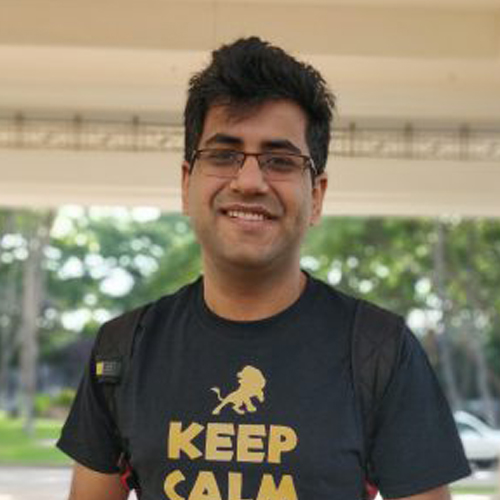
\includegraphics[width=\linewidth]{figures/mohit.jpg}
        \end{subfigure}
        \begin{subfigure}[c]{0.17\textwidth}
            \centering
            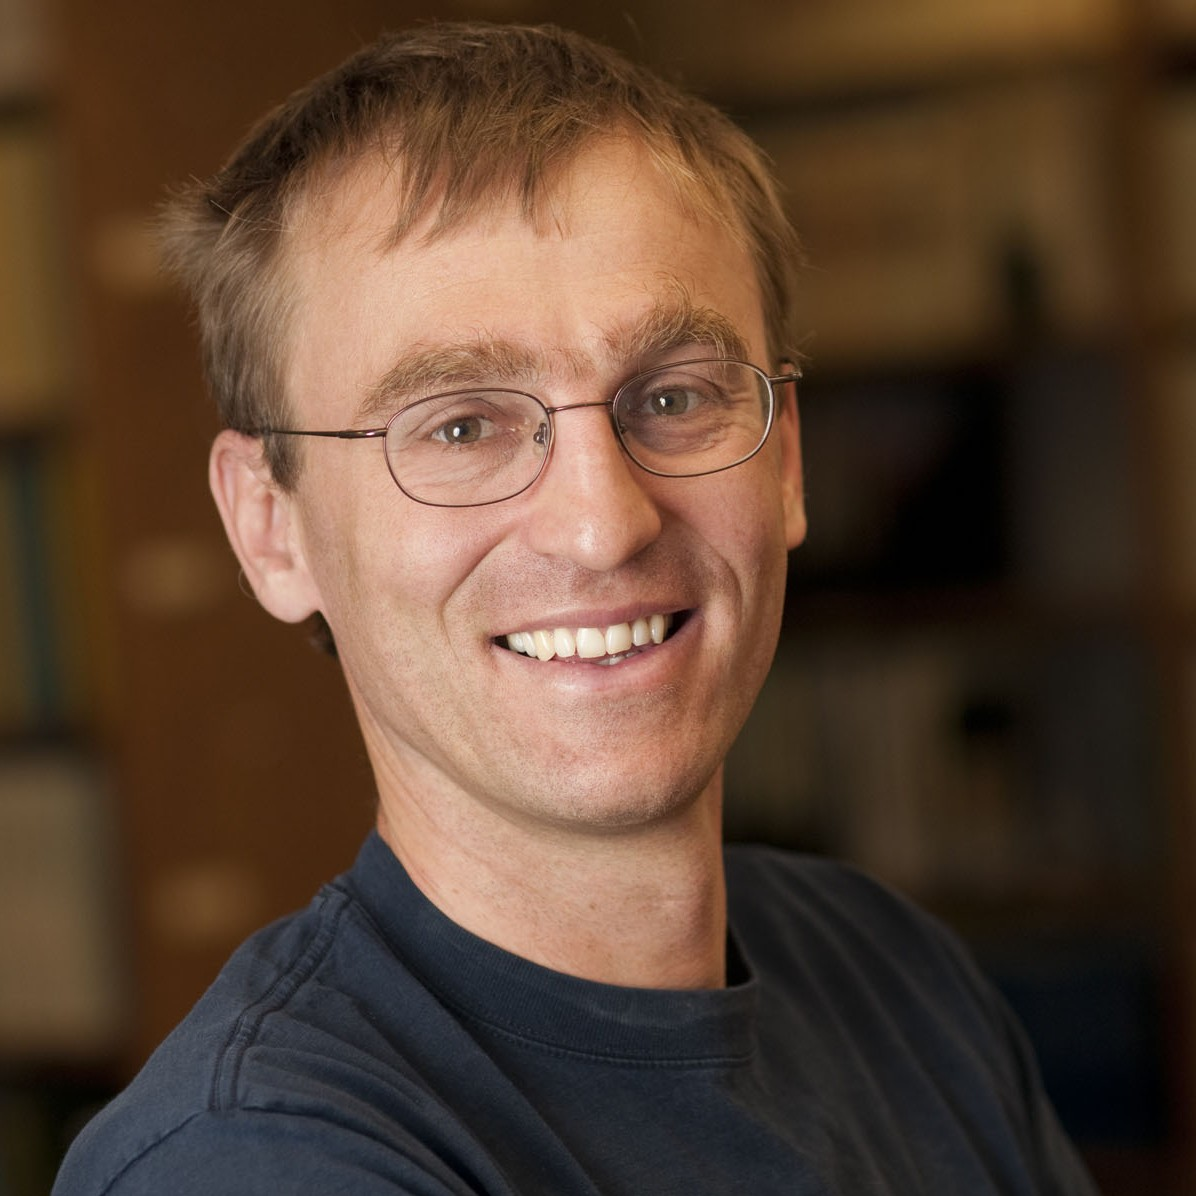
\includegraphics[width=\linewidth]{figures/Tomas.jpg}
        \end{subfigure}

        \begin{subfigure}{0.45\textwidth}
            \centering
            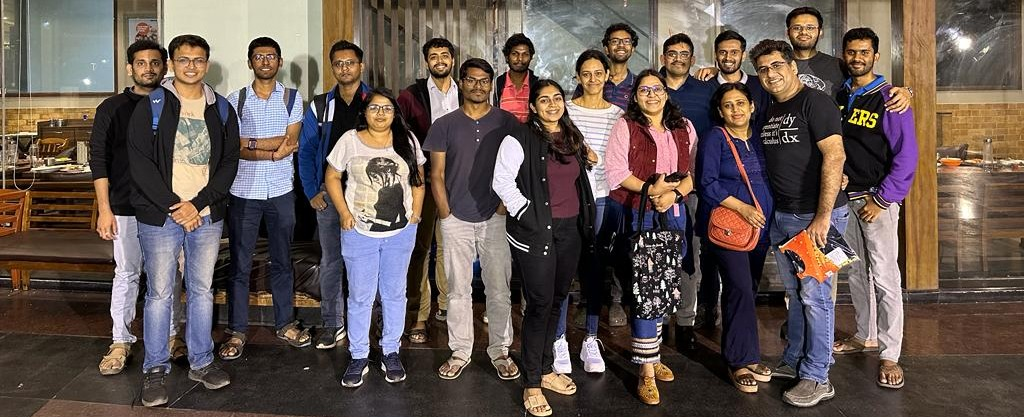
\includegraphics[width=\textwidth]{CSB_Lab}
        \end{subfigure}        
        \begin{subfigure}{0.45\textwidth}
            \centering
            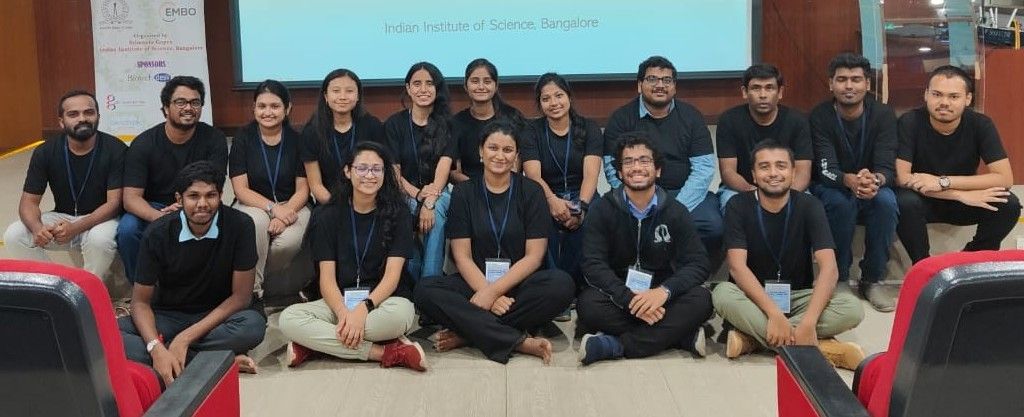
\includegraphics[width=\textwidth]{SG_Lab}
        \end{subfigure}

        \begin{subfigure}[c]{0.15\textwidth}
            \centering
            
\includegraphics[width=0.9\linewidth]{figures/IISc_Seal_Master_logo_Black.pdf}
        \end{subfigure}
        \begin{subfigure}[c]{0.2\textwidth}
            \centering
            
\includegraphics[width=0.9\linewidth]{figures/MSU.png}
        \end{subfigure}
        \begin{subfigure}[c]{0.3\textwidth}
            \centering
            
\includegraphics[width=0.9\linewidth]{PMRF_Logo}
        \end{subfigure}
        \begin{subfigure}[c]{0.15\textwidth}
            \centering
            
\includegraphics[width=0.9\linewidth]{PHPLogo}
        \end{subfigure}
        \begin{subfigure}[c]{0.12\textwidth}
            \centering
            
\includegraphics[width=0.9\textwidth]{figures/afrl.png}
        \end{subfigure}
    \end{figure}
    \end{adjustwidth}        
    \end{frame}

\begin{frame}[standout]
    \Huge{Thank You}
\end{frame}

\begin{frame}[standout]
    Online soon on bioRxiv: 738161
\end{frame}

\end{document}
